\documentclass[conference]{IEEEtran}
\IEEEoverridecommandlockouts
\usepackage{graphicx}
\usepackage{amsmath, amssymb, amsthm}
\usepackage{lipsum}  %
\usepackage{xcolor}
\usepackage{caption}
\usepackage{subcaption}
\usepackage{booktabs} 
\usepackage{hyperref} 
\usepackage{csquotes} 
\usepackage{array}  % 
\usepackage{multirow} 

\newcommand{\customsubcap}[1]{\caption{\fontsize{8}{9}\selectfont #1}}
\newcommand{\figref}[1]{Figure~\ref{#1}}
\newcommand{\tabref}[1]{Table~\ref{#1}}
\newcommand{\secref}[1]{Section~\ref{#1}}
\newcommand{\vv}[1]{\boldsymbol{#1}}
\newcommand{\mat}[1]{\mathbf{#1}}

\newcommand{\todo}[1]{\textcolor{red}{TODO: #1}}
\newcommand{\thre}{\text{th}} 
\newcommand{\subfire}{\text{f}}
\newcommand{\supinit}{\text{init}}
\newcommand{\gt}{\text{gt}}
\newcommand{\pgt}{\text{pgt}}
\usepackage{cite}
\usepackage{amsmath,amssymb,amsfonts}
\usepackage{algorithmic}
\usepackage{graphicx}
\usepackage{textcomp}
\usepackage{xcolor}
\def\BibTeX{{\rm B\kern-.05em{\sc i\kern-.025em b}\kern-.08em
    T\kern-.1667em\lower.7ex\hbox{E}\kern-.125emX}}

\newcommand{\revise}[1]{\textcolor{black}{#1}}
\newcommand{\blockRevise}{\color{black}}

\begin{document}

\title{Prediction of the Most Fire-Sensitive Point in Building Structures with Differentiable Agents for Thermal Simulators}

\author{
    \IEEEauthorblockN{Yuan Xinjie}
    \IEEEauthorblockA{Shenzhen International Graduate School\\
        Tsinghua University\\
        Shenzhen, Guangdong, China \&\\
        Pacific Earthquake Engineering Research (PEER) Center \\
        University of California, Berkeley \\
        Berkeley, California, U.S.A \\
        yuanxj23@mails.tsinghua.edu.cn; yuan.xinjie@berkeley.edu
    }

\and
    \IEEEauthorblockN{Khalid M. Mosalam$^*$}
    \IEEEauthorblockA{Pacific Earthquake Engineering Research (PEER) Center \\
        University of California, Berkeley \& \\
        Department of Civil and Environmental Engineering \\
        University of California, Berkeley \\
        Berkeley, California, U.S.A\\
        mosalam@berkeley.edu
    }
}



\maketitle

\let\thefootnote\relax
\footnotetext{Professor Khalid M. Mosalam is the corresponding author. 

This paper is currently under review at \textit{Computer-Aided Civil and Infrastructure Engineering}.}

\begin{abstract}
\begin{abstract}  
Test time scaling is currently one of the most active research areas that shows promise after training time scaling has reached its limits.
Deep-thinking (DT) models are a class of recurrent models that can perform easy-to-hard generalization by assigning more compute to harder test samples.
However, due to their inability to determine the complexity of a test sample, DT models have to use a large amount of computation for both easy and hard test samples.
Excessive test time computation is wasteful and can cause the ``overthinking'' problem where more test time computation leads to worse results.
In this paper, we introduce a test time training method for determining the optimal amount of computation needed for each sample during test time.
We also propose Conv-LiGRU, a novel recurrent architecture for efficient and robust visual reasoning. 
Extensive experiments demonstrate that Conv-LiGRU is more stable than DT, effectively mitigates the ``overthinking'' phenomenon, and achieves superior accuracy.
\end{abstract}  
\end{abstract}

\begin{IEEEkeywords}
Differentiable agents, Finite Element Analysis, Graph Neural Networks, Most Fire-Sensitive Point,  Structural stability, Thermal simulation.
\end{IEEEkeywords}

\section{Introduction}


\begin{figure}[t]
\centering
\includegraphics[width=0.6\columnwidth]{figures/evaluation_desiderata_V5.pdf}
\vspace{-0.5cm}
\caption{\systemName is a platform for conducting realistic evaluations of code LLMs, collecting human preferences of coding models with real users, real tasks, and in realistic environments, aimed at addressing the limitations of existing evaluations.
}
\label{fig:motivation}
\end{figure}

\begin{figure*}[t]
\centering
\includegraphics[width=\textwidth]{figures/system_design_v2.png}
\caption{We introduce \systemName, a VSCode extension to collect human preferences of code directly in a developer's IDE. \systemName enables developers to use code completions from various models. The system comprises a) the interface in the user's IDE which presents paired completions to users (left), b) a sampling strategy that picks model pairs to reduce latency (right, top), and c) a prompting scheme that allows diverse LLMs to perform code completions with high fidelity.
Users can select between the top completion (green box) using \texttt{tab} or the bottom completion (blue box) using \texttt{shift+tab}.}
\label{fig:overview}
\end{figure*}

As model capabilities improve, large language models (LLMs) are increasingly integrated into user environments and workflows.
For example, software developers code with AI in integrated developer environments (IDEs)~\citep{peng2023impact}, doctors rely on notes generated through ambient listening~\citep{oberst2024science}, and lawyers consider case evidence identified by electronic discovery systems~\citep{yang2024beyond}.
Increasing deployment of models in productivity tools demands evaluation that more closely reflects real-world circumstances~\citep{hutchinson2022evaluation, saxon2024benchmarks, kapoor2024ai}.
While newer benchmarks and live platforms incorporate human feedback to capture real-world usage, they almost exclusively focus on evaluating LLMs in chat conversations~\citep{zheng2023judging,dubois2023alpacafarm,chiang2024chatbot, kirk2024the}.
Model evaluation must move beyond chat-based interactions and into specialized user environments.



 

In this work, we focus on evaluating LLM-based coding assistants. 
Despite the popularity of these tools---millions of developers use Github Copilot~\citep{Copilot}---existing
evaluations of the coding capabilities of new models exhibit multiple limitations (Figure~\ref{fig:motivation}, bottom).
Traditional ML benchmarks evaluate LLM capabilities by measuring how well a model can complete static, interview-style coding tasks~\citep{chen2021evaluating,austin2021program,jain2024livecodebench, white2024livebench} and lack \emph{real users}. 
User studies recruit real users to evaluate the effectiveness of LLMs as coding assistants, but are often limited to simple programming tasks as opposed to \emph{real tasks}~\citep{vaithilingam2022expectation,ross2023programmer, mozannar2024realhumaneval}.
Recent efforts to collect human feedback such as Chatbot Arena~\citep{chiang2024chatbot} are still removed from a \emph{realistic environment}, resulting in users and data that deviate from typical software development processes.
We introduce \systemName to address these limitations (Figure~\ref{fig:motivation}, top), and we describe our three main contributions below.


\textbf{We deploy \systemName in-the-wild to collect human preferences on code.} 
\systemName is a Visual Studio Code extension, collecting preferences directly in a developer's IDE within their actual workflow (Figure~\ref{fig:overview}).
\systemName provides developers with code completions, akin to the type of support provided by Github Copilot~\citep{Copilot}. 
Over the past 3 months, \systemName has served over~\completions suggestions from 10 state-of-the-art LLMs, 
gathering \sampleCount~votes from \userCount~users.
To collect user preferences,
\systemName presents a novel interface that shows users paired code completions from two different LLMs, which are determined based on a sampling strategy that aims to 
mitigate latency while preserving coverage across model comparisons.
Additionally, we devise a prompting scheme that allows a diverse set of models to perform code completions with high fidelity.
See Section~\ref{sec:system} and Section~\ref{sec:deployment} for details about system design and deployment respectively.



\textbf{We construct a leaderboard of user preferences and find notable differences from existing static benchmarks and human preference leaderboards.}
In general, we observe that smaller models seem to overperform in static benchmarks compared to our leaderboard, while performance among larger models is mixed (Section~\ref{sec:leaderboard_calculation}).
We attribute these differences to the fact that \systemName is exposed to users and tasks that differ drastically from code evaluations in the past. 
Our data spans 103 programming languages and 24 natural languages as well as a variety of real-world applications and code structures, while static benchmarks tend to focus on a specific programming and natural language and task (e.g. coding competition problems).
Additionally, while all of \systemName interactions contain code contexts and the majority involve infilling tasks, a much smaller fraction of Chatbot Arena's coding tasks contain code context, with infilling tasks appearing even more rarely. 
We analyze our data in depth in Section~\ref{subsec:comparison}.



\textbf{We derive new insights into user preferences of code by analyzing \systemName's diverse and distinct data distribution.}
We compare user preferences across different stratifications of input data (e.g., common versus rare languages) and observe which affect observed preferences most (Section~\ref{sec:analysis}).
For example, while user preferences stay relatively consistent across various programming languages, they differ drastically between different task categories (e.g. frontend/backend versus algorithm design).
We also observe variations in user preference due to different features related to code structure 
(e.g., context length and completion patterns).
We open-source \systemName and release a curated subset of code contexts.
Altogether, our results highlight the necessity of model evaluation in realistic and domain-specific settings.





The advancement of artificial intelligence in the legal domain has led to the development of various tools that assist in legal research, document retrieval, and automated legal reasoning. Several studies have explored the use of Natural Language Processing (NLP)\cite{khurana2023natural}, machine learning models, and vector-based search mechanisms to enhance the efficiency of legal chatbots. The primary focus of this literature review is on retrieval-augmented generation (RAG) models, FAISS-based document retrieval, deep learning for legal applications, and the use of large language models (LLMs) in legal AI.  

Recent research on Retrieval-Augmented Generation (RAG)\cite{gao2023retrieval} for legal AI has demonstrated its potential in enhancing legal text retrieval and summarization. S. S. Manathunga, Y. and A. Illangasekara\cite{manathunga2023retrieval} proposed a RAG-based model that improves legal text summarization by dynamically fetching relevant documents before generating responses. Similarly, Lee and Ryu \cite{ryu-etal-2023-retrieval} explored the application of RAG in case law retrieval, demonstrating its superiority over traditional keyword-based search engines. The introduction of RAG has significantly improved response accuracy by grounding AI-generated text in authoritative legal documents, reducing hallucinations in AI-driven legal assistance.  

% \begin{figure}[h]
%     \centering
%     \includegraphics[width=8cm]{FAISS.png}
%     \caption{Faiss: Efficient Similarity Search and Clustering of Dense Vectors}
%     \label{Overall Result of comparing FAISS and Chroma with different number of top documents}
% \end{figure}

The efficiency of FAISS (Facebook AI Similarity Search) in legal document retrieval has also been widely studied. Zhao et al. \cite{devlin-etal-2019-bert} implemented FAISS to enhance large-scale legal question answering systems, achieving significant improvements in retrieval speed and relevance. N. Goyal and D. Chen \cite{inbook} demonstrated that FAISS-based vector search mechanisms outperform conventional database searches in legal information retrieval, reducing query response time while maintaining high accuracy. The integration of FAISS with transformer-based models, as seen in the work of Hsieh and Wu, further enhances semantic retrieval, ensuring that chatbot responses align with actual legal texts.  

Transformer-based models such as BERT and GPT-based architecture have also contributed to the evolution of AI-driven legal research. Devlin et al. introduced BERT (Bidirectional Encoder Representations from Transformers), which significantly improved the understanding of legal language. RoBERTa, an optimized version of BERT, was later developed by Liu et al. \cite{liu2019roberta} to enhance contextual understanding and document similarity matching in legal queries. These models have been integrated into legal chatbots for contract analysis and legal decision-making, as demonstrated in the studies of Li et al. and Jin and Liu, where fine-tuned transformers improved legal text comprehension and summarization.  
The role of deep learning in legal AI has also been investigated extensively. Radford et al. introduced GPT-3, which paved the way for legal AI assistants capable of generating human-like responses. However, researchers such as Firth and Lee emphasized the limitations of LLMs in legal reasoning, arguing that these models require external verification mechanisms to prevent misinformation. The use of contrastive learning and fine-tuning for legal text retrieval has been explored by Arabi and Akbari \cite{article}, who demonstrated that embedding-based retrieval significantly improves chatbot response accuracy.  

Another significant area of research involves evaluating AI-generated legal responses using automated metrics. Zhang and Wu introduced BLEU\cite{10.3115/1073083.1073135} and ROUGE\cite{lin-2004-rouge} scores as a means to evaluate AI-generated legal text summaries, ensuring their quality and relevance. Similarly, Zhao et al. \cite{yuan2024rag} examined the effectiveness of RAG-based models in handling complex legal queries, highlighting the importance of legal consistency scores (LCS) in evaluating AI-driven responses.  

The practical applications of legal AI chatbots have been studied extensively in the context of access to justice and AI ethics. Wang and Cheng et al. \cite{xue2024bias} highlighted the potential of AI-driven legal assistants in bridging the justice gap, particularly in countries where legal resources are not easily accessible. Chan conducted a systematic review of retrieval-based legal chatbots, noting that while these systems improve accessibility, they also raise ethical concerns regarding legal misinformation and bias. Research by Min \cite{Min2023ARTIFICIALIA} explored methods for bias detection and mitigation in legal AI, ensuring fairness in AI-generated legal advice.  

Comparative studies between rule-based legal bots, keyword-driven legal search engines, and AI-powered legal chatbots further illustrate the superiority of retrieval-augmented approaches. In a study conducted by Zeng \cite{zeng2024scalable}, FAISS-based retrieval mechanisms significantly outperformed traditional Boolean keyword searches, reducing irrelevant document retrieval by 40\%. Singh \cite{10760929} further demonstrated that AI-powered legal research tools using NLP provide faster and more contextually accurate responses compared to standard legal databases.  

Despite these advancements, challenges remain in AI-driven legal research. Existing chatbots still struggle with multi-jurisdictional legal queries, as noted by Weichbroth \cite{Weichbroth2025AIAT}, who emphasized the need for jurisdiction-aware legal AI models. Additionally, legal AI models often lack the ability to process long-context legal arguments effectively, a limitation discussed by Gupta, who proposed memory-based retrieval techniques to improve long-form legal text processing.  

Research continues to refine AI-driven legal assistance, particularly in retrieval-augmented generation, FAISS-based search, transformer models, and deep learning techniques for legal research. However, further improvements are needed in bias mitigation, jurisdiction-specific adaptations, and long-context legal understanding. Future developments in multilingual legal AI, enhanced retrieval mechanisms, and AI-powered contract analysis will be crucial in making legal AI tools more accessible, reliable, and widely applicable in legal practice.
\begin{teaserfigure}
    \centering
    \includegraphics[width=1\linewidth]{figures/hero_fig.png}
    \caption{Our system translates English text into a photorealistic ASL video with non-manual information. It starts with an English text input (first row), generates ASL tokens capturing both manual and non-manual details (second row), produces a skeletal pose sequence (third row), and finally creates the photorealistic ASL video (fourth row). \han{@all, please check the stylization.}}
    % \han{should we have a longer sentence? Ideally has 6-7 video frames. Still working on stylization...} \rotem{thinking about it again, instead of putting it here, I would have 1-2 examples here- only text->gloss->ours with expressions (or through pose), then have a no expression vs expression fig later on in the paper..}}
    \label{fig:system_overview}
\end{teaserfigure}
\section{MIDR Predictor}
\label{sec:mdrp}
The MIDR predictor functions as a differentiable agent for the FEA simulators. Leveraging GNNs for structural representation, the predictor integrates Transfer Learning (TL) to optimize data utilization while focusing on the MIDR prediction. Additionally, an innovative EU module, to update the edge attributes of the GNNs, is introduced to capture changes in the finite element attributes during fire scenarios.

\subsection{GNNs}
\label{subsec:gnn}

\subsubsection{Overview of GNNs}
Building structures and graphs share an intrinsic similarity: structural nodes correspond to graph nodes, and structural elements (e.g., beams and columns) map naturally to graph edges. This analogy forms the basis for utilizing GNNs in structural data processing. A typical GNN consists of multiple stacked layers, where the output of one layer serves as the input for the next. Each  layer executes three core operations --message passing, aggregation \& update-- expressed as follows:
\begin{equation}
    \label{eq:gnn_overview}
    \vec{v}_i^k = \gamma^k \left( \vec{v}_i^{k-1}, \bigoplus_{j \in \mathcal{N}(i)} \phi^k \left( \vec{v}_i^{k-1}, \vec{v}_j^{k-1}, \vec{e}_{j,i} \right) \right),
\end{equation}
where $\gamma^k(\cdot)$ and $\phi^k(\cdot)$ represent the update and message functions, respectively, $\bigoplus$ is the aggregation operation, e.g., sum, mean, or max, $\mathcal{N}(i)$ denotes the set of neighboring nodes of node $i$, and $\vec{v}_i^k$ and $\vec{e}_{j,i}$ are the attributes of node $i$ at the $k$-th layer and of the edge from node $j$ to node $i$, respectively. Here, both $\gamma^k(\cdot)$ and $\phi^k(\cdot)$ are Multi-Layer Perceptrons (MLPs), i.e., fully connected NNs. \revise{The operations $\gamma(\cdot) ,\phi(\cdot) \, \& \, \bigoplus$ are not related to certain nodes or edges, indicating that the GNN architecture inherently supports variable-sized graphs through parameter-sharing mechanisms. Each graph is processed independently, with identical NN operations applied to all nodes and edges regardless of their number.} \figref{fig:gnn_illustration} is a schematic of a GNN with $K$ layers, illustrating the role of node and edge encoders, as well as the EU mechanism. The shown GNN incorporates initial node and edge encoders to transform the input features into higher-dimensional spaces and utilizes an EU mechanism to dynamically update the edge attributes during each layer to capture changes of the finite elements during fire scenarios.
\begin{figure*}[h!]
    \centering
    \includegraphics[width=1\linewidth]{figures/gnn_illustration.pdf}
    \caption{Illustration of a $K$-layer GNN architecture, demonstrating information flow within the network for a graph with $N$ nodes.}
    \label{fig:gnn_illustration}
\end{figure*}

\subsubsection{Input attributes}
\label{subsubsec:input_attributes}
In our framework, gravity and thermal loads are applied to the beams and columns. These elements dictate the information encapsulated in the nodes and edges of the graph representation.

\paragraph{Node attributes} 
% The information associated with each node $i$ in the structure includes geometric details, specifically the 3D coordinates $(x_i, y_i, z_i)$. These coordinates are essential for representing the spatial configuration of the structure. % Additionally, since floor height, $h_i$, is a critical factor in fire scenarios, it is also included as a key node attribute.
\revise{The coordinates of the $i$-th node in 3 Dimensions (3D) $(x_i, y_i, z_i)$, essential to represent the spatial configuration of the structure, are included as node attributes. Additionally, its floor level $h_i$, a critical factor to define the fire scenarios, is included as another node attribute. For ease of description, we call the four-tuple $\left(x_i, y_i, z_i, h_i\right)$ extended coordinates of node $i$. To account for the fire location, the extended coordinates of the fire source $\left(x_{\subfire}, y_{\subfire}, z_{\subfire}, h_{\subfire}\right)$, containing the 3D coordinates and the corresponding floor level of the fire, are incorporated into the node attributes. Note that $h_i$ and $h_{\subfire}$ are integers.
To enhance the model's ability to capture fire-related information, we compute the differences between the node's and fire source's extended coordinates $\left(x_i - x_{\subfire}, y_i - y_{\subfire}, z_i - z_{\subfire}, h_i - h_{\subfire}\right)$.
Finally, the Euclidean distance between the $i$-th node and the fire location is calculated as $\sqrt{(x_i-x_{\subfire})^2 + (y_i-y_{\subfire})^2 + (z_i - z_{\subfire})^2}$. 
% according to Equation (\ref{eq:Ls}) with $x=x_i$, $y=y_i$, and $z=z_i$.
These features collectively form the initial attributes of each node $i$, denoted as $\vec{v}_{i}^{\supinit}$, comprising a total of 13 features, i.e., $4$ for the extended coordinates of node $i$, $4$ for the extended coordinates of fire source, $4$ for the differences between these two sets of the extended coordinates, and $1$ for the Euclidean distance.
}

\paragraph{Edge attributes} The edges between nodes represent the structural elements (beams and columns) and encapsulate the following attributes:
\begin{itemize}
    \item {\bf{Material properties}}: Young's modulus \& yield strength at ambient temperature, and the strain-hardening ratio, \revise{counting up to 3 dimensions.}
    \item {\bf{Geometric properties}}: Length, floor level, and element orientation. Note that the orientation is encoded using a {\em{one-hot representation}} for alignment along the $x$-axis, $y$-axis, or $z$-axis. \revise{Therefore, the geometric properties count up to 5 dimensions. In this study and for simplicity, we use square sections for the beams and columns, requiring no additional attributes for the orientation of these sections.}
    \item {\bf{Gravity loads}}: {\revise{The magnitude of the applied load on the element counts as the 9-th dimension.}}
\end{itemize}
The initial attributes of each edge $(i,j)$, denoted as $\vec{e}_{i,j}^{\supinit}$, are represented by 9-dimensional vector combining these three sets of attributes.

\paragraph{Feature encoding} The raw node and edge attributes are not directly input into the GNN. Instead,  encoders are employed to map the initial attributes into higher-dimensional spaces, which improve the model's ability for feature representation as follows: 
\begin{itemize}
    \item {\bf{Node encoder}}: Extends the 13-dimensional node attributes $\vec{v}_{i}^{\supinit}$ to $\vec{v}_{i}^0$ with a higher dimensionality, e.g., 64 dimensions. The superscript $0$ indicates it is the input of the first GNN layer.
    \item {\bf{Edge encoder}}: Maps the 9-dimensional edge attributes $\vec{e}_{i,j}^{\supinit}$ to $\vec{e}_{i,j}$ with a higher-dimensional representation, e.g., 32 dimensions. 
\end{itemize}
\revise{
After extending the dimensions of node and edge features using encoders, their dimensions remain consistent across different layers of the GNN. This simplifies the architecture of the NN design, where different layers have similar structures, all with the same input and output dimensions. This characteristic of unchanged dimensions allows for the ease of extracting edge or node features from any layer of the GNN and performing the same processing for the MIDR prediction, as detailed in \secref{subsubsec:handle_structural_data}. If we do not use encoders to expand the dimensions and instead maintain consistent dimensions across different layers of the GNN, i.e., node attributes remain at 13 dimensions, the model capacity decreases and the performance of the predictor accordingly declines.
}
% These encoders, implemented as simple single-hidden-layer MLPs, ensures that the feature dimensions across different layers remain consistent. This consistency is crucial because the number of GNN layers a structure passes through is determined by its maximum number of stories, consistent dimensionality allows for seamless information flow and extraction across layers. This hierarchical encoding approach ensures that the GNN effectively captures the structural and fire-related information necessary for accurate MIDR predictions.

\subsubsection{Handling structural data}
\label{subsubsec:handle_structural_data}
A significant challenge in GNNs is the {\em{over-smoothing}}, where during each layer's update process, a node's attributes aggregate information from its neighboring nodes. Consequently, increasing the number of layers causes node attributes to homogenize, losing their specificity and  negatively impacting the model's performance. This issue is particularly pronounced in building structures with varying story counts and number of nodes, such as 2-story vs. 7-story buildings. If both are passed through a 7-layer GNN, the node attributes of the 2-story building would experience severe over-smoothing. 
\revise{
In simple terms, when there are too many message-passing layers, the characteristics of all nodes tend to be consistent. However, too few layers lead to the problem of incomplete perception, i.e., nodes cannot obtain information from distant nodes.
}
To mitigate this problem, we adopt the method from \cite{chou_structgnn_2024}, restricting the number of GNN layers for each graph, i.e., building structure herein, to the building's number of stories. 
\revise{
In this way, the number of layers is properly set, neither too many nor too few, ensuring that critical information about fire propagation is retained in the node attributes without over-smoothing.
}

Beams and columns exhibit distinct load characteristics that influence how they are represented in graph-based model of a structure. Beams primarily bear gravity loads that act perpendicular to their span direction, which aligns with their structural function in predominantly resisting bending moments and shear forces. Under thermal expansion due to fire, these loads affect both end nodes of the beam. As a result, when representing beams in a graph model, it is intuitive to treat them as {\em{undirected edges}}, reflecting their bidirectional influence on the connected nodes. {\revise{Columns, on the other hand, experience gravity loads along their axial direction, directed downward, which is consistent with their role in mainly supporting vertical loads in addition to bending moments and shear forces due to their frame action with the floor beams}}. When a column deforms under loads (due to thermal expansion, lateral loads, or gravity), the displacements at any point in the column influence the displacements above it, which continues sequentially upward along the column length. However, in the mathematical formulation of the FEA, the computation involves solving global system of equations that inherently account for all inter-dependencies between elements and boundary conditions simultaneously, not sequentially. Accordingly, representing columns as {\em{directed edges}} might initially seem appropriate, as it allows separate transmission of force and displacement information. However, in GNNs, undirected graphs are commonly implemented by duplicating directed edges and reversing their directions to ensure bidirectional information flow. Given this practical implementation in GNNs, both beams and columns are treated as {\bf{undirected edges}} in our graph model. This approach simplifies the representation while preserving the necessary information flow for structural analysis.

\subsubsection{Edge update mechanism}
\label{subsubsec:edge_update}
Typically GNNs often do not update edge attributes, $\vec{e}_{i,j}$, during the iterative update process in each layer. However, in the context of fire scenarios, the attributes of beams and columns (e.g., material properties and geometrical characteristics) evolve with temperature changes, directly affecting the MIDR computations. To address this need, we introduce an EU module that dynamically updates edge attributes during each layer's computation. After updating node attributes via message passing in each layer of the GNN, the EU module utilizes the attributes of the two adjacent nodes and the edge itself to update the edge attributes. This ensures that the edge features reflect the ongoing structural changes due to fire conditions. 

With the EU module, the standard GNN operation in Equation \eqref{eq:gnn_overview} is modified to include EUs. The updated node attributes are expressed as follows:
\begin{equation}
    \label{eq:gnn_with_edge_update}
    \vec{v}_i^k = \gamma^k \left( \vec{v}_i^{k-1}, \bigoplus_{j \in \mathcal{N}(i)} \phi^k \left( \vec{v}_i^{k-1}, \vec{v}_j^{k-1}, \vec{e}_{j,i}^{k-1} \right) \right).
\end{equation}
The EU module updates the edge attributes as follows:
\begin{equation}
    \label{eq:edge_update}
    \vec{e}_{j,i}^k = \zeta \left( \vec{v}_i^{k}, \vec{v}_j^{k} \right) + \vec{e}_{j,i}^{k-1},
\end{equation}
where $\zeta(\cdot)$ is the update function for edge attributes, implemented as a single-hidden-layer MLP. The inclusion of the EU module enables:
\begin{enumerate}
    \item {\bf{Dynamic adaptation}}: Capture temperature-induced changes in beam and column properties during each GNN layer's computations.
    \item {\bf{Enhanced modeling}}: Simultaneously updates node and edge attributes, resulting in a more accurate representation of the structural state.
    \item {\bf{Improved performance}}: Provides the GNN with the ability to better model the structural transformations under fire scenarios, leading to more precise MIDR predictions.
\end{enumerate}    
By iteratively updating edge attributes, the EU module effectively integrates the evolving structural properties into the GNN, enhancing its predictive capabilities in fire scenarios.

\subsection{TL-based Network Training}
\label{subsec:transfer_learning}
\revise{The proposed GNN framework only computes an embedding vector for each node. Therefore, to obtain the predicted MIDR, additional operations (layers) are needed. Two straightforward methods to aggregate the node-level results to a graph-level prediction can be applied. These two baseline methods are referred to as Strawman 1 \& 2 and they only differ in where and what to aggregate, as discussed below:}
% To predict the IDR, an additional MLP is employed to map the node embedding vector to the corresponding IDR value. We explore two baseline training and inference methods, referred to as Strawman 1 and Strawman 2, as illustrated in \figref{fig:transfer_learning}:
\begin{itemize}
    \item {\textbf{Strawman 1}} \revise{aggregates the node embeddings in a graph into a single graph embedding, using a {\em{pooling operation}}, which predicts MIDR with an additional MLP.}
    \item {\textbf{Strawman 2}} \revise{predicts the IDR of each node using node embeddings and an additional MLP. Then it aggregates node-level IDR predictions by selecting MIDR from them.}
    % the IDR for each node is directly predicted using its embedding, and the maximum value is selected as the structure's MIDR.
\end{itemize}

While Strawman 1 focuses solely on predicting the MIDR, it fails to leverage the IDR labels available for individual node data. Consequently, this approach risks overfitting when the dataset is small. On the other hand, Strawman 2 uses all node-level IDR labels, but the inclusion of non-MIDR nodes during training may dilute the model's focus on predicting the MIDR. To overcome these limitations, we propose a TL-based training method that integrates the strengths of both approaches. By framing the problem as two related tasks --predicting node-level IDRs and structure-level MIDR-- we adopt a multi-task TL approach with a two-step training procedure, \figref{fig:transfer_learning}. 
\begin{figure}[h!]
    \centering
    \includegraphics[width=1\linewidth]{figures/transfer_learning.pdf}
    \caption{Different training strategies (head-1 \& head-2 are MLPs for different tasks, e.g., predicting IDR of each node in a structure and MIDR of the structure.}
    \label{fig:transfer_learning}
\end{figure}

In the first step, the GNN is trained to predict the IDR of individual nodes, using an MLP referred to as {\bf{task head-1}} as in Strawman 2, \figref{fig:transfer_learning}. During this step, the GNN learns to extract global structural features. The loss function for this step is defined as follows:
\begin{equation}
    \label{eq:mdr_loss_task1}
    \begin{aligned}
        & L_{\text{task-1}}\left(\Theta_{\text{GNN}}, \Theta_{\text{head-1}}\right)\\
        & \qquad=\frac{1}{\sum_{m=1}^{M} N_{m} I_{m}}\sum_{m=1}^{M} \sum_{n=1}^{N_{m}} \sum_{i=1}^{I_{m}} \left( d_{m,n,i}^{\, \gt} - \widehat{d}_{m,n,i} \right)^2,
    \end{aligned}
\end{equation}  
where $d_{m,n,i}^{\, \gt}$ is the ground truth IDR for node $i \in \left(1,2,\dots,I_{m}\right)$ in structure $m \in (1,2,\dots,M)$ computed via OpenSeesRT under fire scenario $n \in \left(1,2,\dots,N_{m}\right)$, $\widehat{d}_{m,n,i}$ is the predicted IDR from the model, $\Theta_{\text{GNN}}$ is the set of parameters of the GNN, and $\Theta_{\text{head-1}}$ is the set of parameters of task head-1. The optimization objective for this step is as follows:  
\begin{equation}
    \label{eq:mdr_task1}
    \min_{\Theta_{\text{GNN}}, \Theta_{\text{head-1}}} L_{\text{task-1}}\left(\Theta_{\text{GNN}}, \Theta_{\text{head-1}}\right).
\end{equation}  

In the second step, the trained GNN parameters from the first step are reused as a {\em{feature extractor}}. The MLP for node-level IDR prediction (task head-1) is replaced with a new MLP, referred to as {\bf{task head-2}} as in Strawman 1, \figref{fig:transfer_learning}, to predict the structure MIDR. During this step, task head-2 is first trained independently, followed by {\em{fine-tuning}} the entire GNN. The MIDR for structure $m$ under fire scenario $n$ is defined as:  
\begin{equation}
    d_{m,n,\max} \triangleq \max_{i=1,2,\dots,I_{m}} d_{m,n,i}.
\end{equation}  
The loss function for this step is defined as follows:
\begin{equation}
    \label{eq:mdr_loss_task2}
    \begin{aligned}
        & L_{\text{task-2}}\left(\Theta_{\text{GNN}}, \Theta_{\text{head-2}}\right)\\
        & \qquad=\frac{1}{\sum_{m=1}^{M} N_{m}}\sum_{m=1}^{M} \sum_{n=1}^{N_{m}} \left( d_{m,n,\max}^{\, \gt} - \widehat{d}_{m,n,\max} \right)^2,
    \end{aligned}
\end{equation}  
where $d_{m,n,\max}^{\, \gt}$ is the ground truth MIDR for structure $m$ under fire scenario $n$ computed using OpenSeesRT, $\widehat{d}_{m,n,\max}$ is the predicted MIDR from the model, and $\Theta_{\text{head-2}}$ is the set of parameters of task head-2. The optimization objective for this step is as follows:
\begin{equation}
    \label{eq:mdr_task2}
    \min_{\Theta_{\text{GNN}}, \Theta_{\text{head-2}}} L_{\text{task-2}}\left(\Theta_{\text{GNN}}, \Theta_{\text{head-2}}\right).
\end{equation}  

The proposed TL-based methods offers these benefits:
\begin{enumerate}
    \item {\bf{Effective utilization of data}}: Leverages node-level IDR labels while focusing on MIDR prediction.
    \item {\bf{Improved generalization}}: Enhances the model's ability to generalize across diverse fire scenarios and structural configurations.
    \item {\bf{Accurate MIDR predictions}}: Integrates global structural information for precise MIDR predictions, outperforming the individual Strawman methods 1 \& 2.
\end{enumerate}
By combining node-level and structure-level predictions in a two-step training pipeline, the TL-based approach achieves a robust balance between learning granular details and capturing global structural patterns. 

\section{MFSP Predictor}
\label{sec:mfspp}

With the training of the MIDR predictor complete, we have developed a NN-based agent model that effectively serves as a surrogate for the FEA conducted using OpenSeesRT. This agent model presents two critical advantages over traditional FEA: (1) computational efficiency and (2) differentiability. These advantages are fully leveraged in training the MFSP predictor, designed to identify the location within the building structure that exhibits the highest vulnerability under fire conditions via the MIDR. Importantly, the training process for the MFSP predictor no longer depends on direct FEA results. Instead, the fixed parameters of the pretrained MIDR predictor are utilized as the computational platform. This allows the MIDR predictor to remain unchanged during the MFSP predictor's training, ensuring consistency and efficiency in the workflow. By relying solely on the outputs of the MIDR predictor, the MFSP predictor benefits from the speed and differentiability of the agent model while eliminating the need for repeated computationally expensive FEA simulations.

\subsection{Pseudo-Labeling and Loss Choice}
\label{subsec:mfspp_pseudo_label}
As illustrated in \figref{fig:system_overview}, the MFSP predictor operates as the ``argmaxer'' of the MIDR predictor. An intuitive choice of the loss function is to minimize the negative output of the MIDR predictor $L_{\text{MIDR}}$. This loss leverages the differentiable nature of the MIDR predictor as an agent. It is expressed as:  
\begin{equation}
    L_{\text{MIDR}} = - \frac{1}{\sum_{m}^{M}N_{m}}\sum_{m}^{M}\sum_{n}^{N_m} \widehat{d}_{m,n,\max}.
\end{equation}
This approach conceptually resembles the Actor-Critic framework in RL \cite{sutton2018reinforcement} where the MFSP predictor is the ``Actor'', proposing actions in the form of fire points, while the MIDR predictor is the ``Critic'', evaluating the quality of the Actor's actions. However, similar to challenges in RL, this method can lead to poor training outcome or convergence issues. MIDR predictor is a complex function and optimizing its output using gradient descent often results in local optima or unstable training. Additionally, the fixed nature of MIDR predictor limits the ability to introduce randomness for balancing exploration and exploitation, a core mechanism in RL.

To address these issues, we propose an alternative approach inspired by the computational efficiency of the MIDR predictor. Instead of directly using $L_{\text{MIDR}}$, we use the MIDR predictor to generate {\em{pseudo ground truths}} for the MFSP. This process is depicted in \figref{fig:pseudo_label}. Specifically, at the granularity of the rooms, we consider the center point of each room in a building as a potential fire point. The MIDR predictor estimates the MIDR for each fire point, and the one with the highest MIDR is selected as the pseudo ground truth MFSP for the building. This pseudo-labeling approach allows efficient labeling of unlabeled data at the room-level granularity.
\begin{figure*}[h!]
    \centering
    \includegraphics[width=1\linewidth]{figures/pseudo_label.pdf}
    \caption{Procedure of pseudo-labeling for building structure $m$.}
    \label{fig:pseudo_label}
\end{figure*}

For a given building structure $m$, let the pseudo ground truth MFSP coordinates be $\left( x_{m}^{\, \pgt}, y_{m}^{\, \pgt}, z_{m}^{\, \pgt}\right)$, with the corresponding MIDR $\widehat{d}_{m}^{\, \pgt}$. Using this pseudo-labeling, we define the Mean Squared Error (MSE) loss as follows:  
\begin{equation}
    \begin{aligned}
        L_{\text{MSE}} = \frac{1}{M}\sum_{m=1}^{M}&\left( \left( x_{m}^{\, \pgt} - \widehat{x}_{m} \right)^2 + \left( y_{m}^{\, \pgt} - \widehat{y}_{m} \right)^2 \right. \\  
        & \left.+ \left( z_{m}^{\, \pgt} - \widehat{z}_{m} \right)^2 \right),
    \end{aligned}
    \label{eq:MSE}
\end{equation}
where $\widehat{x}_{m}$, $\widehat{y}_{m}$, and $\widehat{z}_{m}$ are the MFSP predictor's outputs for structure $m$. Since the pseudo-labeling process provides ground truth at room-level granularity, it is beneficial to combine $L_{\text{MIDR}}$ and $L_{\text{MSE}}$ into a hybrid loss function via a weighted sum to train the MFSP predictor. In this way, the combined loss $L_{\text{Hybrid}}$ is defined as follows:  
\begin{equation}
    L_{\text{Hybrid}} = w_1 \, L_{\text{MIDR}} + w_2 \, L_{\text{MSE}},
    \label{eq:hybrid}
\end{equation}  
where $w_1$ and $w_2$ are weights balancing the contributions of the two loss components. In this study, we fix $w_2=1$, so that $w_1$ is interpreted as a measure of the distrust on the pseudo ground truth MFSP generated by the labeling process. This distrust increases as $w_1$ increases. This hybrid approach combines the strengths of leveraging differentiability through $L_{\text{MIDR}}$ and the guidance provided by pseudo ground truth through $L_{\text{MSE}}$, offering a robust method for training the MFSP predictor.

\subsection{TL with GNN in MIDR Predictor}
\label{subsec:mfspp_transfer_learning}
The MFSP predictor operates as an ``argmaxer'' for the MIDR predictor. While it could be designed as a completely new network and trained from scratch (i.e., De novo training), we propose leveraging the pretrained GNN module from the MIDR predictor through TL. The GNN module in the MIDR predictor captures comprehensive global structural information, making it a suitable platform for the MFSP predictor. Specifically, we reuse the GNN module as a feature extractor, replace the MLP task head with a new one tailored for the MFSP task, and fine-tune the entire model to optimize its performance.
% \subsubsection{Structural information via TL}
By reusing the pretrained GNN module, which encodes essential structural and gravity load features, the MFSP predictor can focus on learning the relationships necessary to identify the MFSP. This approach reduces training time and enhances model performance by building on the already-learned representations of the structural information, rather than starting from scratch.

% \paragraph*{The virtual fire point method}
% \subsubsection{The virtual fire point method}
\revise{A unique challenge arises when reusing the GNN in the MIDR predictor requiring a fire point as the input although not need for the MFSP prediction. Common practice to deal with such problem is {\em{masking}}, especially in computer vision or natural language processing. However, masking, such as zero-value masking (i.e., ignore certain inputs by setting them to zero), cannot be directly applied here, because the 3D coordinates $(0,0,0)$ represent a valid location --a possible fire at the bottom corner of the building structure.} To overcome this challenge, we introduce a randomized Virtual Fire Point (VFP). \revise{Essentially, this VFP can be regarded as a placeholder for the GNN input.} During training, a random virtual fire location is assigned to each structure for every iteration, independently of prior iterations. This randomized approach forces the network to learn the global structural features necessary for predicting the MFSP, while effectively ignoring the influence of specific fire locations. 
In the inference stage, different from training stage, we set the VFP to be the geometric center of the structure, i.e., not being randomized. This ensures that the MSFP predictor focuses on the overall structural information rather than being biased by the presence of specific fire locations. By combining TL and the VFP, the MFSP predictor achieves robust generalization and improved accuracy in identifying the MFSP in diverse structural configurations.

\section{Dataset}
\label{sec:dataset}

\subsection{Data Collection}

To analyze political discussions on Discord, we followed the methodology in \cite{singh2024Cross-Platform}, collecting messages from politically-oriented public servers in compliance with Discord's platform policies.

Using Discord's Discovery feature, we employed a web scraper to extract server invitation links, names, and descriptions, focusing on public servers accessible without participation. Invitation links were used to access data via the Discord API. To ensure relevance, we filtered servers using keywords related to the 2024 U.S. elections (e.g., Trump, Kamala, MAGA), as outlined in \cite{balasubramanian2024publicdatasettrackingsocial}. This resulted in 302 server links, further narrowed to 81 English-speaking, politics-focused servers based on their names and descriptions.

Public messages were retrieved from these servers using the Discord API, collecting metadata such as \textit{content}, \textit{user ID}, \textit{username}, \textit{timestamp}, \textit{bot flag}, \textit{mentions}, and \textit{interactions}. Through this process, we gathered \textbf{33,373,229 messages} from \textbf{82,109 users} across \textbf{81 servers}, including \textbf{1,912,750 messages} from \textbf{633 bots}. Data collection occurred between November 13th and 15th, covering messages sent from January 1st to November 12th, just after the 2024 U.S. election.

\subsection{Characterizing the Political Spectrum}
\label{sec:timeline}

A key aspect of our research is distinguishing between Republican- and Democratic-aligned Discord servers. To categorize their political alignment, we relied on server names and self-descriptions, which often include rules, community guidelines, and references to key ideologies or figures. Each server's name and description were manually reviewed based on predefined, objective criteria, focusing on explicit political themes or mentions of prominent figures. This process allowed us to classify servers into three categories, ensuring a systematic and unbiased alignment determination.

\begin{itemize}
    \item \textbf{Republican-aligned}: Servers referencing Republican and right-wing and ideologies, movements, or figures (e.g., MAGA, Conservative, Traditional, Trump).  
    \item \textbf{Democratic-aligned}: Servers mentioning Democratic and left-wing ideologies, movements, or figures (e.g., Progressive, Liberal, Socialist, Biden, Kamala).  
    \item \textbf{Unaligned}: Servers with no defined spectrum and ideologies or opened to general political debate from all orientations.
\end{itemize}

To ensure the reliability and consistency of our classification, three independent reviewers assessed the classification following the specified set of criteria. The inter-rater agreement of their classifications was evaluated using Fleiss' Kappa \cite{fleiss1971measuring}, with a resulting Kappa value of \( 0.8191 \), indicating an almost perfect agreement among the reviewers. Disagreements were resolved by adopting the majority classification, as there were no instances where a server received different classifications from all three reviewers. This process guaranteed the consistency and accuracy of the final categorization.

Through this process, we identified \textbf{7 Republican-aligned servers}, \textbf{9 Democratic-aligned servers}, and \textbf{65 unaligned servers}.

Table \ref{tab:statistics} shows the statistics of the collected data. Notably, while Democratic- and Republican-aligned servers had a comparable number of user messages, users in the latter servers were significantly more active, posting more than double the number of messages per user compared to their Democratic counterparts. 
This suggests that, in our sample, Democratic-aligned servers attract more users, but these users were less engaged in text-based discussions. Additionally, around 10\% of the messages across all server categories were posted by bots. 

\subsection{Temporal Data} 

Throughout this paper, we refer to the election candidates using the names adopted by their respective campaigns: \textit{Kamala}, \textit{Biden}, and \textit{Trump}. To examine how the content of text messages evolves based on the political alignment of servers, we divided the 2024 election year into three periods: \textbf{Biden vs Trump} (January 1 to July 21), \textbf{Kamala vs Trump} (July 21 to September 20), and the \textbf{Voting Period} (after September 20). These periods reflect key phases of the election: the early campaign dominated by Biden and Trump, the shift in dynamics with Kamala Harris replacing Joe Biden as the Democratic candidate, and the final voting stage focused on electoral outcomes and their implications. This segmentation enables an analysis of how discourse responds to pivotal electoral moments.

Figure \ref{fig:line-plot} illustrates the distribution of messages over time, highlighting trends in total messages volume and mentions of each candidate. Prior to Biden's withdrawal on July 21, mentions of Biden and Trump were relatively balanced. However, following Kamala's entry into the race, mentions of Trump surged significantly, a trend further amplified by an assassination attempt on him, solidifying his dominance in the discourse. The only instance where Trump’s mentions were exceeded occurred during the first debate, as concerns about Biden’s age and cognitive abilities temporarily shifted the focus. In the final stages of the election, mentions of all three candidates rose, with Trump’s mentions peaking as he emerged as the victor.
\definecolor{darkgreen}{rgb}{0.0, 0.5, 0.0}
\definecolor{violet}{rgb}{0.56, 0.0, 1.0}
\section{Evaluation}
We apply our methodology to derive counterfactual policies for various MDPs, addressing three main research questions: (1) how does our policy's performance compare to the Gumbel-max SCM approach; (2) how do the counterfactual stability and monotonicity assumptions impact the probability bounds; and (3) how fast is our approach compared with the Gumbel-max SCM method?

\begin{figure*}
    \centering
    %
    \resizebox{0.6\textwidth}{!}{
        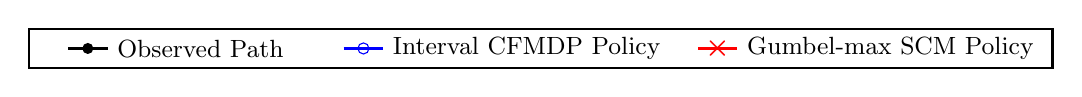
\begin{tikzpicture}[scale=1.0, every node/.style={scale=1.0}]
            \draw[thick, black] (-3, -0.25) rectangle (10, 0.25);
            %
            \draw[black, line width=1pt] (-2.5, 0.0) -- (-2,0.0);
            \fill[black] (-2.25,0.0) circle (2pt); %
            \node[right] at (-2,0.0) {\small Observed Path};
            
            %
            \draw[blue, line width=1pt] (1.0,0.0) -- (1.5,0.0);
            \node[draw=blue, circle, minimum size=4pt, inner sep=0pt] at (1.25,0.0) {}; %
            \node[right] at (1.5,0.0) {\small Interval CFMDP Policy};
            
            %
            \draw[red, line width=1pt] (5.5,0) -- (6,0);
            \node[red] at (5.75,0) {$\boldsymbol{\times}$}; %
            \node[right] at (6,0) {\small Gumbel-max SCM Policy};
        \end{tikzpicture}
    }\\
    %
    \subfigure[\footnotesize Lowest cumulative reward: Interval CFMDP ($312$), Gumbel-max SCM ($312$)]{%
        \resizebox{0.76\columnwidth}{!}{
             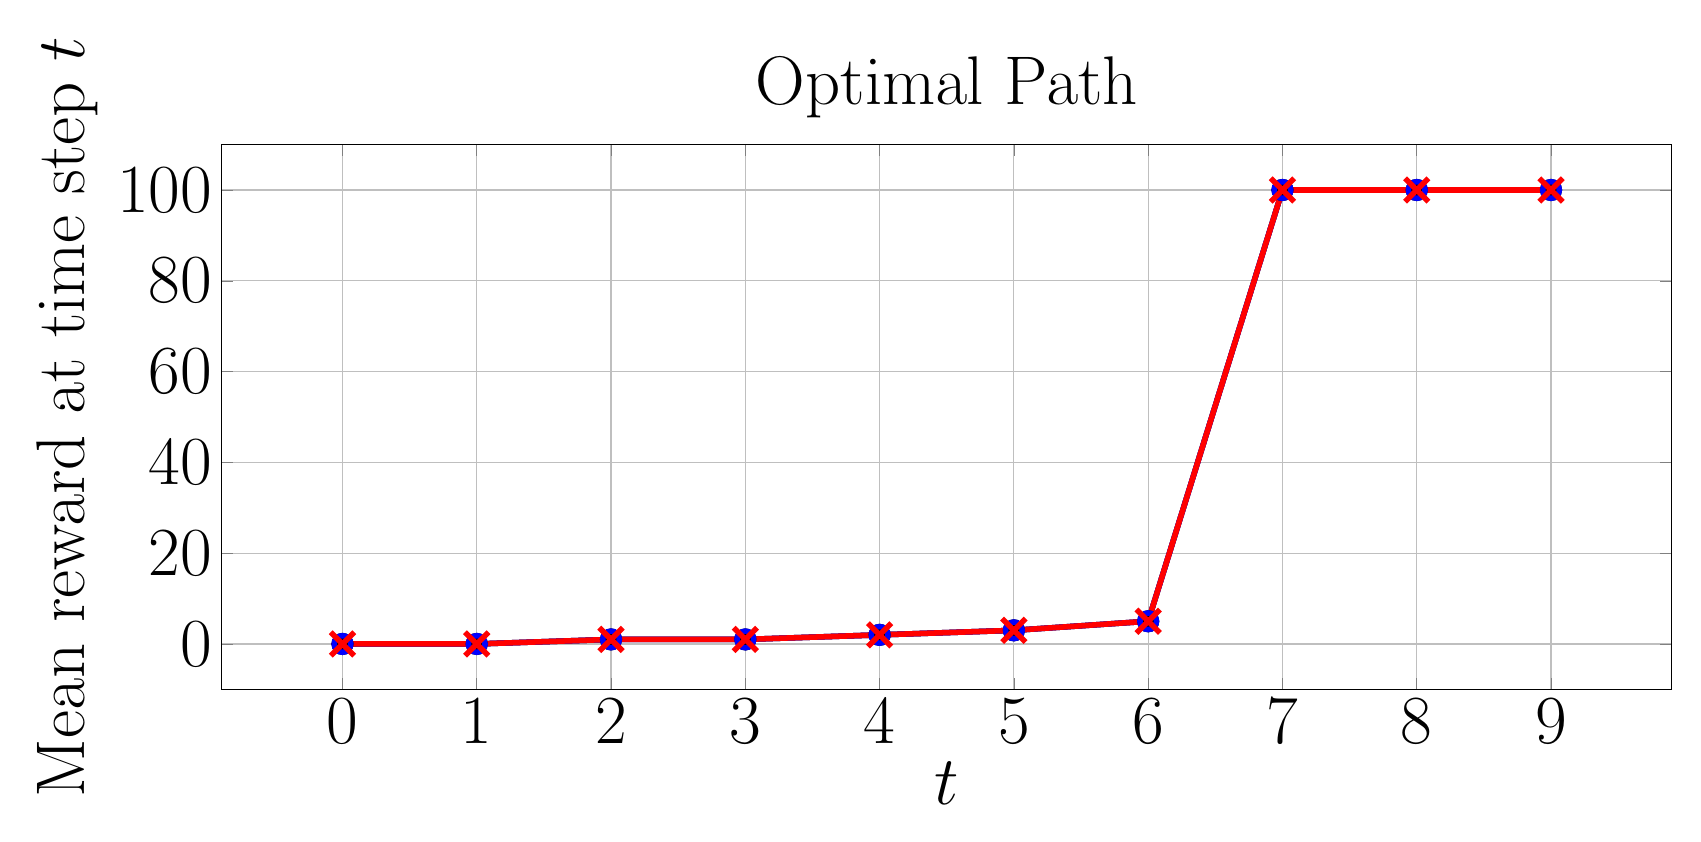
\begin{tikzpicture}
                \begin{axis}[
                    xlabel={$t$},
                    ylabel={Mean reward at time step $t$},
                    title={Optimal Path},
                    grid=both,
                    width=20cm, height=8.5cm,
                    every axis/.style={font=\Huge},
                    %
                ]
                \addplot[
                    color=black, %
                    mark=*, %
                    line width=2pt,
                    mark size=3pt,
                    error bars/.cd,
                    y dir=both, %
                    y explicit, %
                    error bar style={line width=1pt,solid},
                    error mark options={line width=1pt,mark size=4pt,rotate=90}
                ]
                coordinates {
                    (0, 0.0)  +- (0, 0.0)
                    (1, 0.0)  +- (0, 0.0) 
                    (2, 1.0)  +- (0, 0.0) 
                    (3, 1.0)  +- (0, 0.0)
                    (4, 2.0)  +- (0, 0.0)
                    (5, 3.0) +- (0, 0.0)
                    (6, 5.0) +- (0, 0.0)
                    (7, 100.0) +- (0, 0.0)
                    (8, 100.0) +- (0, 0.0)
                    (9, 100.0) +- (0, 0.0)
                };
                %
                \addplot[
                    color=blue, %
                    mark=o, %
                    line width=2pt,
                    mark size=3pt,
                    error bars/.cd,
                    y dir=both, %
                    y explicit, %
                    error bar style={line width=1pt,solid},
                    error mark options={line width=1pt,mark size=4pt,rotate=90}
                ]
                 coordinates {
                    (0, 0.0)  +- (0, 0.0)
                    (1, 0.0)  +- (0, 0.0) 
                    (2, 1.0)  +- (0, 0.0) 
                    (3, 1.0)  +- (0, 0.0)
                    (4, 2.0)  +- (0, 0.0)
                    (5, 3.0) +- (0, 0.0)
                    (6, 5.0) +- (0, 0.0)
                    (7, 100.0) +- (0, 0.0)
                    (8, 100.0) +- (0, 0.0)
                    (9, 100.0) +- (0, 0.0)
                };
                %
                \addplot[
                    color=red, %
                    mark=x, %
                    line width=2pt,
                    mark size=6pt,
                    error bars/.cd,
                    y dir=both, %
                    y explicit, %
                    error bar style={line width=1pt,solid},
                    error mark options={line width=1pt,mark size=4pt,rotate=90}
                ]
                coordinates {
                    (0, 0.0)  +- (0, 0.0)
                    (1, 0.0)  +- (0, 0.0) 
                    (2, 1.0)  +- (0, 0.0) 
                    (3, 1.0)  +- (0, 0.0)
                    (4, 2.0)  +- (0, 0.0)
                    (5, 3.0) +- (0, 0.0)
                    (6, 5.0) +- (0, 0.0)
                    (7, 100.0) +- (0, 0.0)
                    (8, 100.0) +- (0, 0.0)
                    (9, 100.0) +- (0, 0.0)
                };
                \end{axis}
            \end{tikzpicture}
         }
    }
    \hspace{1cm}
    \subfigure[\footnotesize Lowest cumulative reward: Interval CFMDP ($19$), Gumbel-max SCM ($-88$)]{%
         \resizebox{0.76\columnwidth}{!}{
            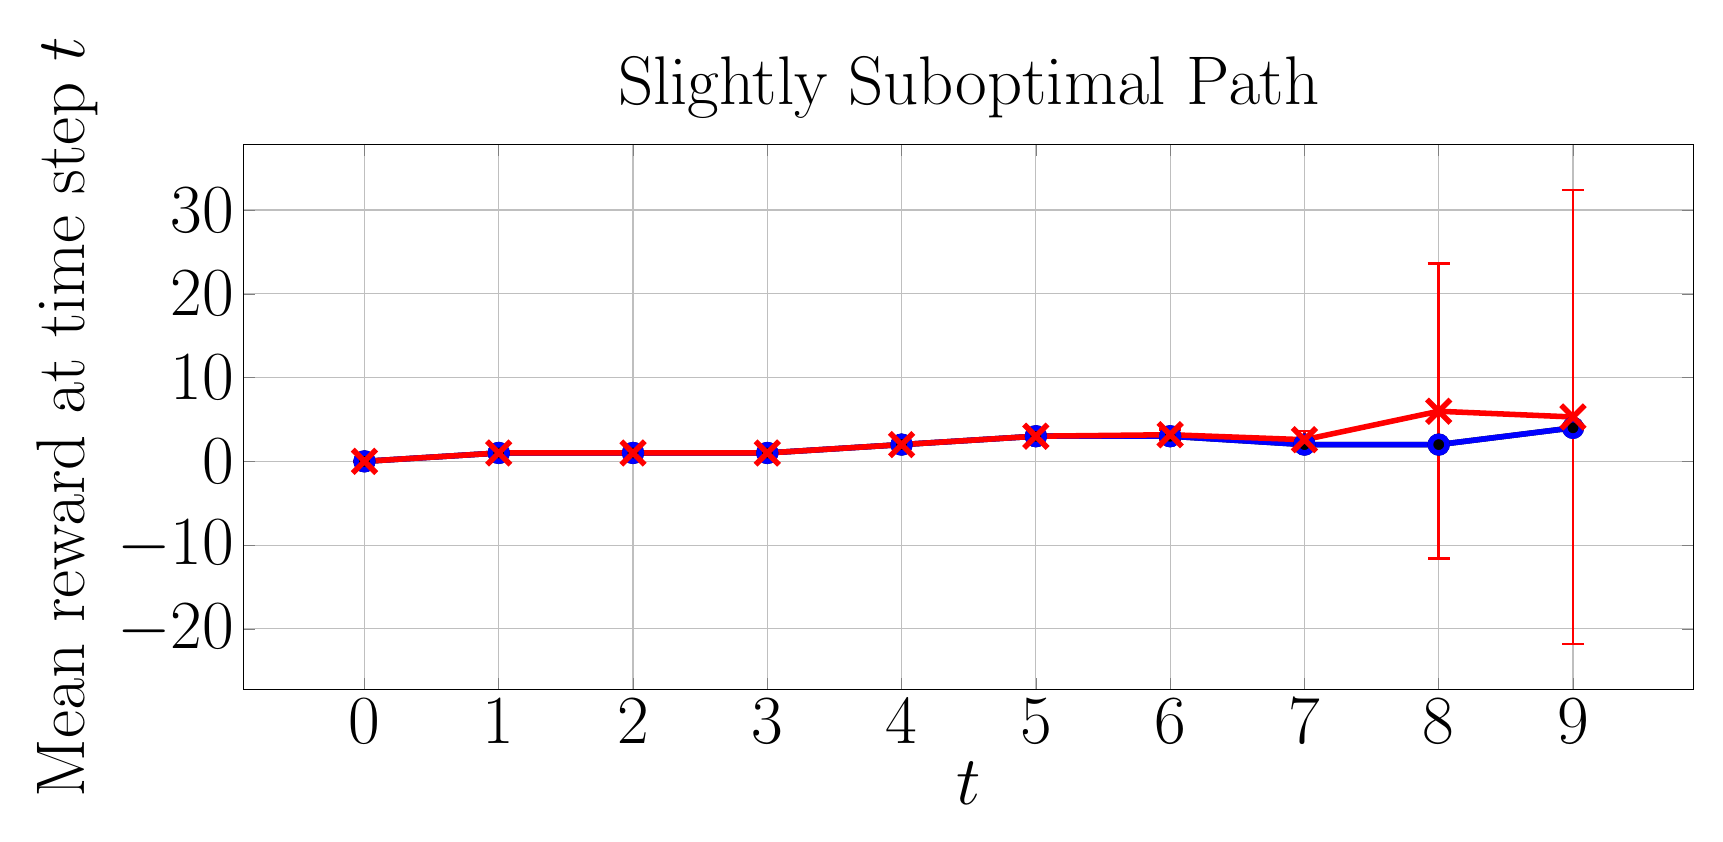
\begin{tikzpicture}
                \begin{axis}[
                    xlabel={$t$},
                    ylabel={Mean reward at time step $t$},
                    title={Slightly Suboptimal Path},
                    grid=both,
                    width=20cm, height=8.5cm,
                    every axis/.style={font=\Huge},
                    %
                ]
                \addplot[
                    color=black, %
                    mark=*, %
                    line width=2pt,
                    mark size=3pt,
                    error bars/.cd,
                    y dir=both, %
                    y explicit, %
                    error bar style={line width=1pt,solid},
                    error mark options={line width=1pt,mark size=4pt,rotate=90}
                ]
              coordinates {
                    (0, 0.0)  +- (0, 0.0)
                    (1, 1.0)  +- (0, 0.0) 
                    (2, 1.0)  +- (0, 0.0) 
                    (3, 1.0)  +- (0, 0.0)
                    (4, 2.0)  +- (0, 0.0)
                    (5, 3.0) +- (0, 0.0)
                    (6, 3.0) +- (0, 0.0)
                    (7, 2.0) +- (0, 0.0)
                    (8, 2.0) +- (0, 0.0)
                    (9, 4.0) +- (0, 0.0)
                };
                %
                \addplot[
                    color=blue, %
                    mark=o, %
                    line width=2pt,
                    mark size=3pt,
                    error bars/.cd,
                    y dir=both, %
                    y explicit, %
                    error bar style={line width=1pt,solid},
                    error mark options={line width=1pt,mark size=4pt,rotate=90}
                ]
              coordinates {
                    (0, 0.0)  +- (0, 0.0)
                    (1, 1.0)  +- (0, 0.0) 
                    (2, 1.0)  +- (0, 0.0) 
                    (3, 1.0)  +- (0, 0.0)
                    (4, 2.0)  +- (0, 0.0)
                    (5, 3.0) +- (0, 0.0)
                    (6, 3.0) +- (0, 0.0)
                    (7, 2.0) +- (0, 0.0)
                    (8, 2.0) +- (0, 0.0)
                    (9, 4.0) +- (0, 0.0)
                };
                %
                \addplot[
                    color=red, %
                    mark=x, %
                    line width=2pt,
                    mark size=6pt,
                    error bars/.cd,
                    y dir=both, %
                    y explicit, %
                    error bar style={line width=1pt,solid},
                    error mark options={line width=1pt,mark size=4pt,rotate=90}
                ]
                coordinates {
                    (0, 0.0)  +- (0, 0.0)
                    (1, 1.0)  +- (0, 0.0) 
                    (2, 1.0)  +- (0, 0.0) 
                    (3, 1.0)  +- (0, 0.0)
                    (4, 2.0)  += (0, 0.0)
                    (5, 3.0)  += (0, 0.0)
                    (6, 3.17847) += (0, 0.62606746) -= (0, 0.62606746)
                    (7, 2.5832885) += (0, 1.04598233) -= (0, 1.04598233)
                    (8, 5.978909) += (0, 17.60137623) -= (0, 17.60137623)
                    (9, 5.297059) += (0, 27.09227512) -= (0, 27.09227512)
                };
                \end{axis}
            \end{tikzpicture}
         }
    }\\[-1.5pt]
    \subfigure[\footnotesize Lowest cumulative reward: Interval CFMDP ($14$), Gumbel-max SCM ($-598$)]{%
         \resizebox{0.76\columnwidth}{!}{
             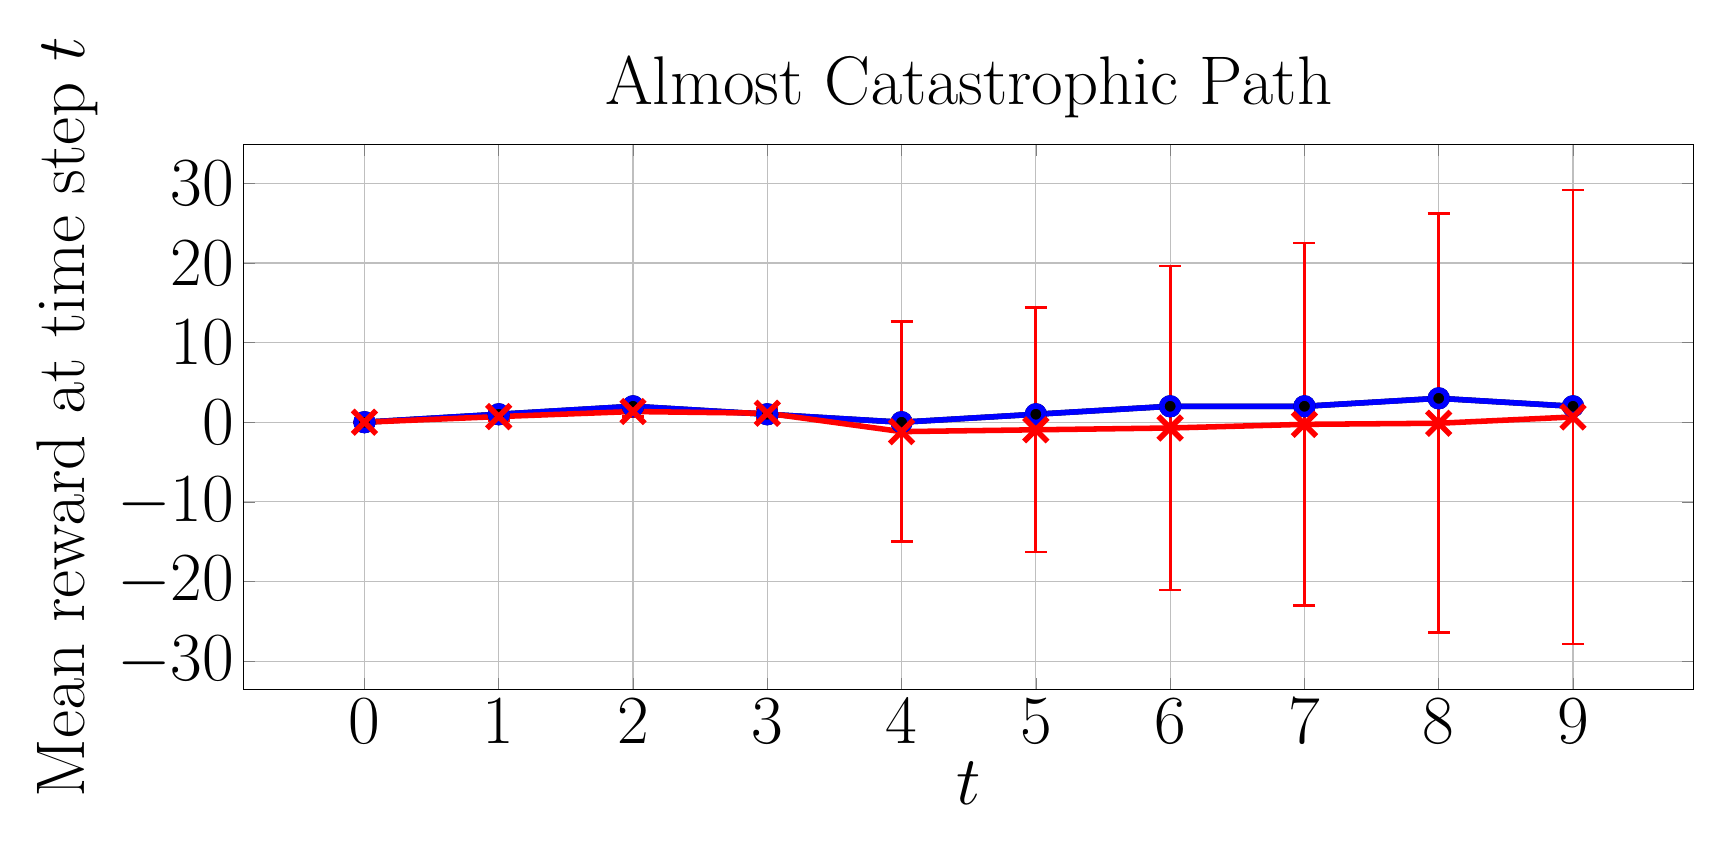
\begin{tikzpicture}
                \begin{axis}[
                    xlabel={$t$},
                    ylabel={Mean reward at time step $t$},
                    title={Almost Catastrophic Path},
                    grid=both,
                    width=20cm, height=8.5cm,
                    every axis/.style={font=\Huge},
                    %
                ]
                \addplot[
                    color=black, %
                    mark=*, %
                    line width=2pt,
                    mark size=3pt,
                    error bars/.cd,
                    y dir=both, %
                    y explicit, %
                    error bar style={line width=1pt,solid},
                    error mark options={line width=1pt,mark size=4pt,rotate=90}
                ]
                coordinates {
                    (0, 0.0)  +- (0, 0.0)
                    (1, 1.0)  +- (0, 0.0) 
                    (2, 2.0)  +- (0, 0.0) 
                    (3, 1.0)  +- (0, 0.0)
                    (4, 0.0)  +- (0, 0.0)
                    (5, 1.0) +- (0, 0.0)
                    (6, 2.0) +- (0, 0.0)
                    (7, 2.0) +- (0, 0.0)
                    (8, 3.0) +- (0, 0.0)
                    (9, 2.0) +- (0, 0.0)
                };
                %
                \addplot[
                    color=blue, %
                    mark=o, %
                    line width=2pt,
                    mark size=3pt,
                    error bars/.cd,
                    y dir=both, %
                    y explicit, %
                    error bar style={line width=1pt,solid},
                    error mark options={line width=1pt,mark size=4pt,rotate=90}
                ]
                coordinates {
                    (0, 0.0)  +- (0, 0.0)
                    (1, 1.0)  +- (0, 0.0) 
                    (2, 2.0)  +- (0, 0.0) 
                    (3, 1.0)  +- (0, 0.0)
                    (4, 0.0)  +- (0, 0.0)
                    (5, 1.0) +- (0, 0.0)
                    (6, 2.0) +- (0, 0.0)
                    (7, 2.0) +- (0, 0.0)
                    (8, 3.0) +- (0, 0.0)
                    (9, 2.0) +- (0, 0.0)
                };
                %
                \addplot[
                    color=red, %
                    mark=x, %
                    line width=2pt,
                    mark size=6pt,
                    error bars/.cd,
                    y dir=both, %
                    y explicit, %
                    error bar style={line width=1pt,solid},
                    error mark options={line width=1pt,mark size=4pt,rotate=90}
                ]
                coordinates {
                    (0, 0.0)  +- (0, 0.0)
                    (1, 0.7065655)  +- (0, 0.4553358) 
                    (2, 1.341673)  +- (0, 0.67091621) 
                    (3, 1.122926)  +- (0, 0.61281824)
                    (4, -1.1821935)  +- (0, 13.82444042)
                    (5, -0.952399)  +- (0, 15.35195457)
                    (6, -0.72672) +- (0, 20.33508414)
                    (7, -0.268983) +- (0, 22.77861454)
                    (8, -0.1310835) +- (0, 26.31013314)
                    (9, 0.65806) +- (0, 28.50670214)
                };
                %
            %
            %
            %
            %
            %
            %
            %
            %
            %
            %
            %
            %
            %
            %
            %
            %
            %
            %
                \end{axis}
            \end{tikzpicture}
         }
    }
    \hspace{1cm}
    \subfigure[\footnotesize Lowest cumulative reward: Interval CFMDP ($-698$), Gumbel-max SCM ($-698$)]{%
         \resizebox{0.76\columnwidth}{!}{
            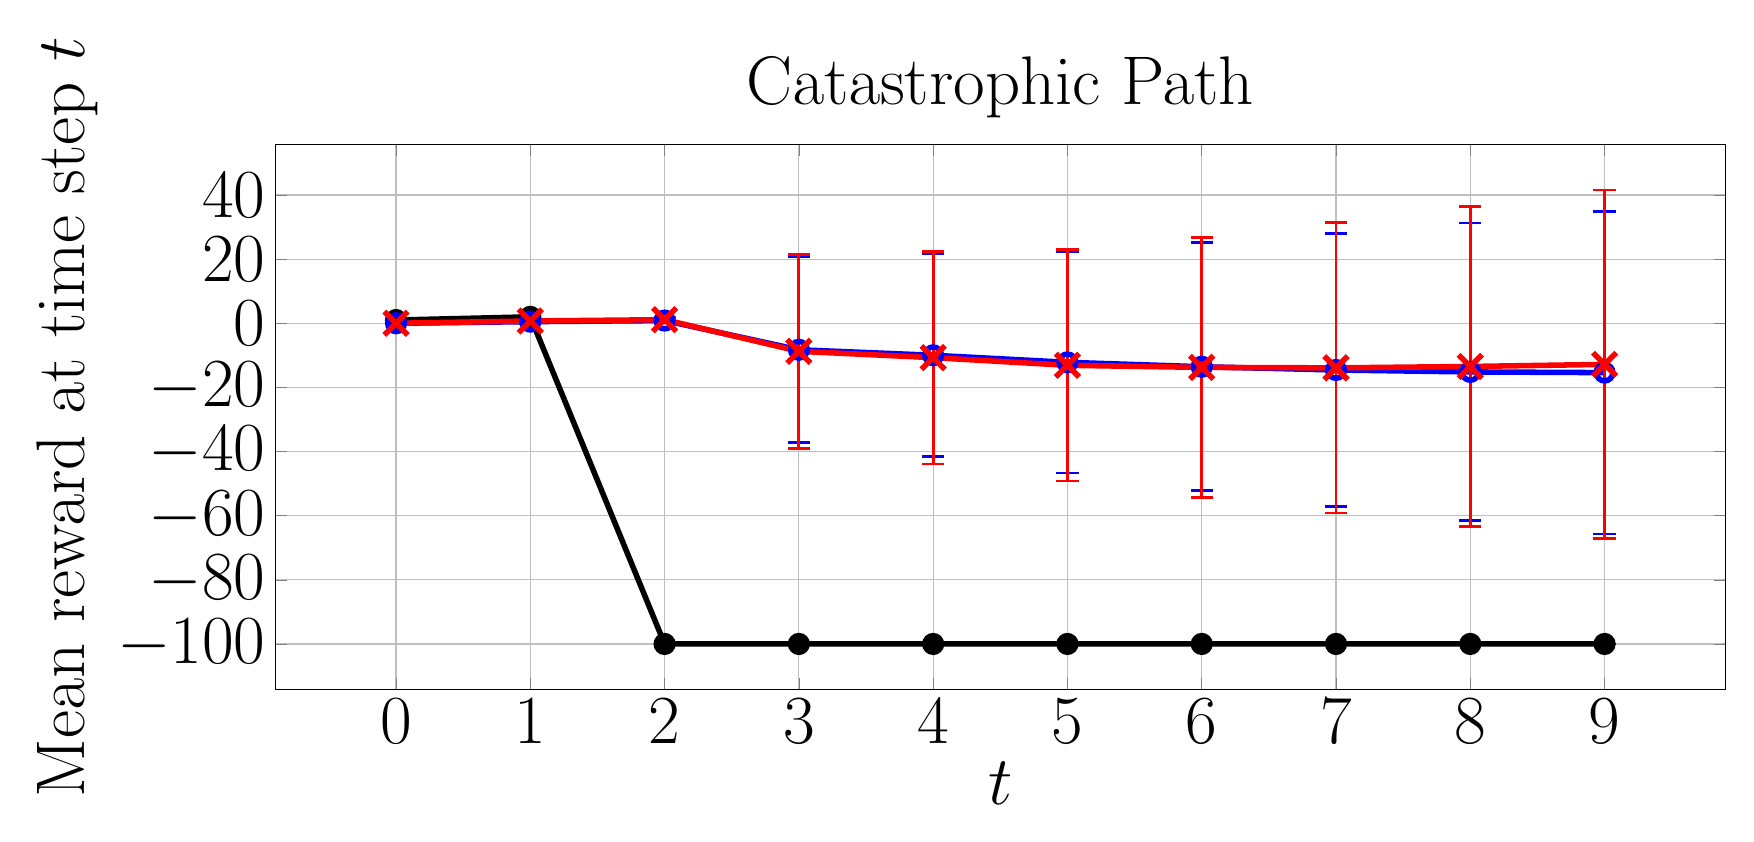
\begin{tikzpicture}
                \begin{axis}[
                    xlabel={$t$},
                    ylabel={Mean reward at time step $t$},
                    title={Catastrophic Path},
                    grid=both,
                    width=20cm, height=8.5cm,
                    every axis/.style={font=\Huge},
                    %
                ]
                \addplot[
                    color=black, %
                    mark=*, %
                    line width=2pt,
                    mark size=3pt,
                    error bars/.cd,
                    y dir=both, %
                    y explicit, %
                    error bar style={line width=1pt,solid},
                    error mark options={line width=1pt,mark size=4pt,rotate=90}
                ]
                coordinates {
                    (0, 1.0)  +- (0, 0.0)
                    (1, 2.0)  +- (0, 0.0) 
                    (2, -100.0)  +- (0, 0.0) 
                    (3, -100.0)  +- (0, 0.0)
                    (4, -100.0)  +- (0, 0.0)
                    (5, -100.0) +- (0, 0.0)
                    (6, -100.0) +- (0, 0.0)
                    (7, -100.0) +- (0, 0.0)
                    (8, -100.0) +- (0, 0.0)
                    (9, -100.0) +- (0, 0.0)
                };
                %
                \addplot[
                    color=blue, %
                    mark=o, %
                    line width=2pt,
                    mark size=3pt,
                    error bars/.cd,
                    y dir=both, %
                    y explicit, %
                    error bar style={line width=1pt,solid},
                    error mark options={line width=1pt,mark size=4pt,rotate=90}
                ]
                coordinates {
                    (0, 0.0)  +- (0, 0.0)
                    (1, 0.504814)  +- (0, 0.49997682) 
                    (2, 0.8439835)  +- (0, 0.76831917) 
                    (3, -8.2709165)  +- (0, 28.93656754)
                    (4, -9.981082)  +- (0, 31.66825363)
                    (5, -12.1776325) +- (0, 34.53463233)
                    (6, -13.556076) +- (0, 38.62845372)
                    (7, -14.574418) +- (0, 42.49603359)
                    (8, -15.1757075) +- (0, 46.41913968)
                    (9, -15.3900395) +- (0, 50.33563368)
                };
                %
                \addplot[
                    color=red, %
                    mark=x, %
                    line width=2pt,
                    mark size=6pt,
                    error bars/.cd,
                    y dir=both, %
                    y explicit, %
                    error bar style={line width=1pt,solid},
                    error mark options={line width=1pt,mark size=4pt,rotate=90}
                ]
                coordinates {
                    (0, 0.0)  +- (0, 0.0)
                    (1, 0.701873)  +- (0, 0.45743556) 
                    (2, 1.1227805)  +- (0, 0.73433129) 
                    (3, -8.7503255)  +- (0, 30.30257976)
                    (4, -10.722092)  +- (0, 33.17618589)
                    (5, -13.10721)  +- (0, 36.0648089)
                    (6, -13.7631645) +- (0, 40.56553451)
                    (7, -13.909043) +- (0, 45.23829402)
                    (8, -13.472517) +- (0, 49.96270296)
                    (9, -12.8278835) +- (0, 54.38618735)
                };
                %
            %
            %
            %
            %
            %
            %
            %
            %
            %
            %
            %
            %
            %
            %
            %
            %
            %
            %
                \end{axis}
            \end{tikzpicture}
         }
    }
    \caption{Average instant reward of CF paths induced by policies on GridWorld $p=0.4$.}
    \label{fig: reward p=0.4}
\end{figure*}

\subsection{Experimental Setup}
To compare policy performance, we measure the average rewards of counterfactual paths induced by our policy and the Gumbel-max policy by uniformly sampling $200$ counterfactual MDPs from the ICFMDP and generating $10,000$ counterfactual paths over each sampled CFMDP. \jl{Since the interval CFMDP depends on the observed path, we select $4$  paths of varying optimality to evaluate how the observed path impacts the performance of both policies: an optimal path, a slightly suboptimal path that could reach the optimal reward with a few changes, a catastrophic path that enters a catastrophic, terminal state with low reward, and an almost catastrophic path that was close to entering a catastrophic state.} When measuring the average probability bound widths and execution time needed to generate the ICFMDPs, we averaged over $20$ randomly generated observed paths
\footnote{Further training details are provided in Appendix \ref{app: training details}, and the code is provided at \href{https://github.com/ddv-lab/robust-cf-inference-in-MDPs}{https://github.com/ddv-lab/robust-cf-inference-in-MDPs}
%
%
.}.

\subsection{GridWorld}
\jl{The GridWorld MDP is a $4 \times 4$ grid where an agent must navigate from the top-left corner to the goal state in the bottom-right corner, avoiding a dangerous terminal state in the centre. At each time step, the agent can move up, down, left, or right, but there is a small probability (controlled by hyper-parameter $p$) of moving in an unintended direction. As the agent nears the goal, the reward for each state increases, culminating in a reward of $+100$ for reaching the goal. Entering the dangerous state results in a penalty of $-100$. We use two versions of GridWorld: a less stochastic version with $p=0.9$ (i.e., $90$\% chance of moving in the chosen direction) and a more stochastic version with $p=0.4$.}

\paragraph{GridWorld ($p=0.9$)}
When $p=0.9$, the counterfactual probability bounds are typically narrow (see Table \ref{tab:nonzero_probs} for average measurements). Consequently, as shown in Figure \ref{fig: reward p=0.9}, both policies are nearly identical and perform similarly well across the optimal, slightly suboptimal, and catastrophic paths.
%
However, for the almost catastrophic path, the interval CFMDP path is more conservative and follows the observed path more closely (as this is where the probability bounds are narrowest), which typically requires one additional step to reach the goal state than the Gumbel-max SCM policy.
%

\paragraph{GridWorld ($p=0.4$)}
\jl{When $p=0.4$, the GridWorld environment becomes more uncertain, increasing the risk of entering the dangerous state even if correct actions are chosen. Thus, as shown in Figure \ref{fig: reward p=0.4}, the interval CFMDP policy adopts a more conservative approach, avoiding deviation from the observed policy if it cannot guarantee higher counterfactual rewards (see the slightly suboptimal and almost catastrophic paths), whereas the Gumbel-max SCM is inconsistent: it can yield higher rewards, but also much lower rewards, reflected in the wide error bars.} For the catastrophic path, both policies must deviate from the observed path to achieve a higher reward and, in this case, perform similarly.
%
%
%
%
\subsection{Sepsis}
The Sepsis MDP \citep{oberst2019counterfactual} simulates trajectories of Sepsis patients. Each state consists of four vital signs (heart rate, blood pressure, oxygen concentration, and glucose levels), categorised as low, normal, or high.
and three treatments that can be toggled on/off at each time step (8 actions in total). Unlike \citet{oberst2019counterfactual}, we scale rewards based on the number of out-of-range vital signs, between $-1000$ (patient dies) and $1000$ (patient discharged). \jl{Like the GridWorld $p=0.4$ experiment, the Sepsis MDP is highly uncertain, as many states are equally likely to lead to optimal and poor outcomes. Thus, as shown in Figure \ref{fig: reward sepsis}, both policies follow the observed optimal and almost catastrophic paths to guarantee rewards are no worse than the observation.} However, improving the catastrophic path requires deviating from the observation. Here, the Gumbel-max SCM policy, on average, performs better than the interval CFMDP policy. But, since both policies have lower bounds clipped at $-1000$, neither policy reliably improves over the observation. In contrast, for the slightly suboptimal path, the interval CFMDP policy performs significantly better, shown by its higher lower bounds. 
Moreover, in these two cases, the worst-case counterfactual path generated by the interval CFMDP policy is better than that of the Gumbel-max SCM policy,
indicating its greater robustness.
%
\begin{figure*}
    \centering
     \resizebox{0.6\textwidth}{!}{
        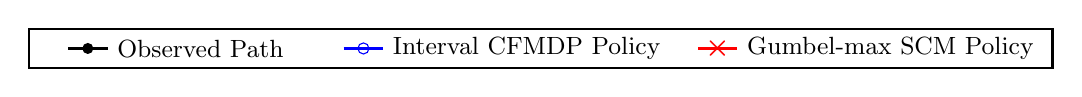
\begin{tikzpicture}[scale=1.0, every node/.style={scale=1.0}]
            \draw[thick, black] (-3, -0.25) rectangle (10, 0.25);
            %
            \draw[black, line width=1pt] (-2.5, 0.0) -- (-2,0.0);
            \fill[black] (-2.25,0.0) circle (2pt); %
            \node[right] at (-2,0.0) {\small Observed Path};
            
            %
            \draw[blue, line width=1pt] (1.0,0.0) -- (1.5,0.0);
            \node[draw=blue, circle, minimum size=4pt, inner sep=0pt] at (1.25,0.0) {}; %
            \node[right] at (1.5,0.0) {\small Interval CFMDP Policy};
            
            %
            \draw[red, line width=1pt] (5.5,0) -- (6,0);
            \node[red] at (5.75,0) {$\boldsymbol{\times}$}; %
            \node[right] at (6,0) {\small Gumbel-max SCM Policy};
        \end{tikzpicture}
    }\\
    \subfigure[\footnotesize Lowest cumulative reward: Interval CFMDP ($8000$), Gumbel-max SCM ($8000$)]{%
         \resizebox{0.76\columnwidth}{!}{
             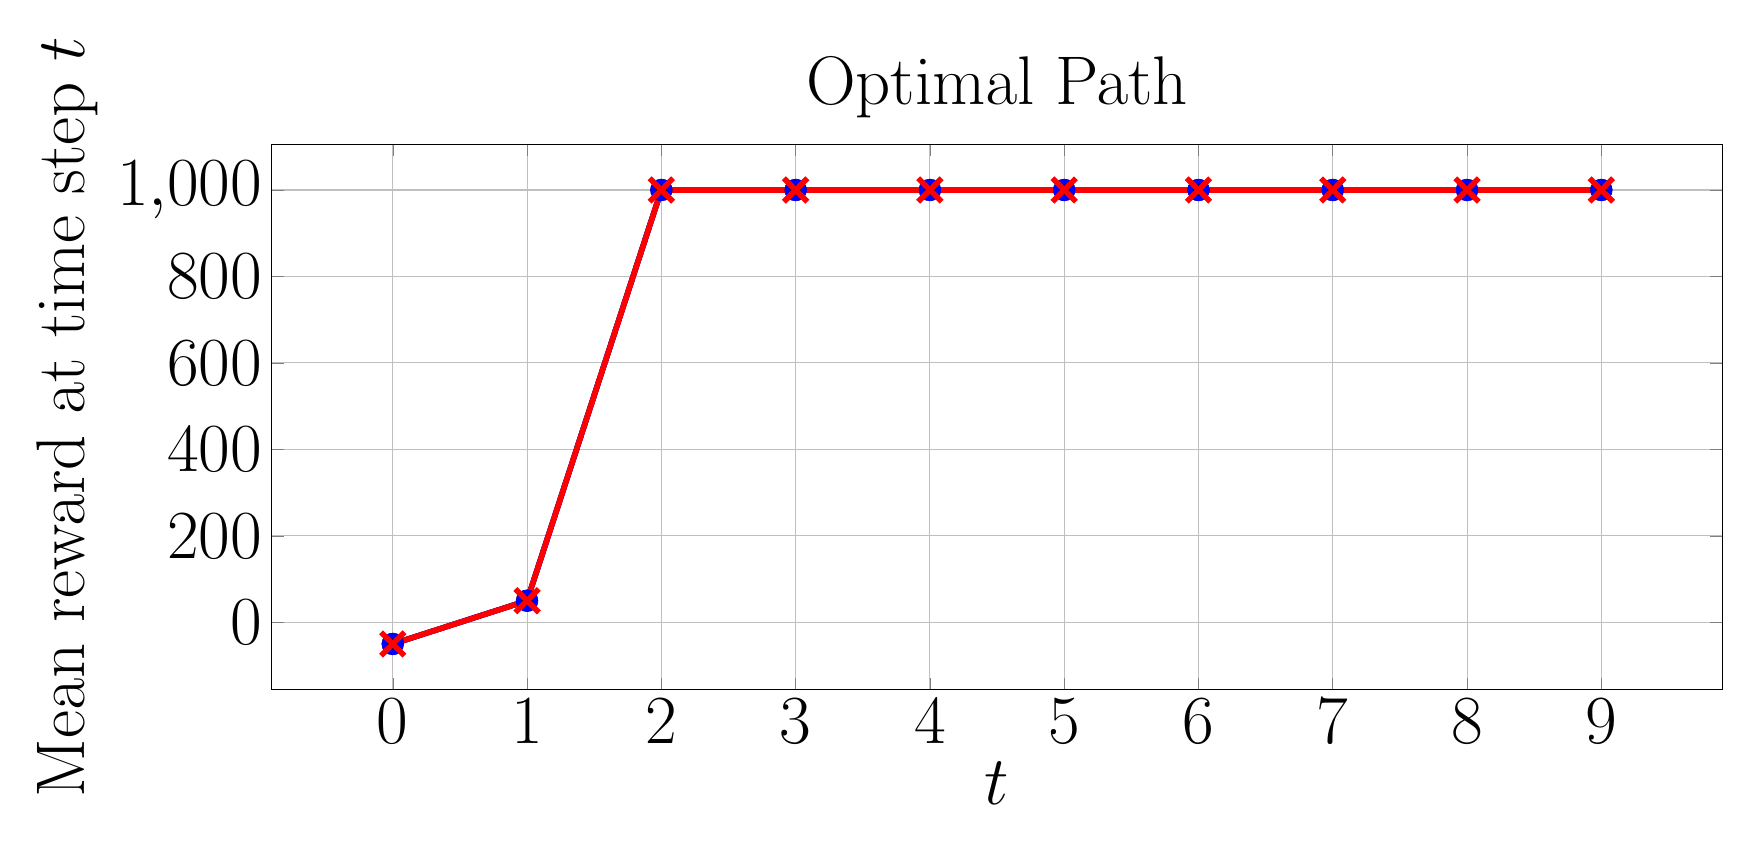
\begin{tikzpicture}
                \begin{axis}[
                    xlabel={$t$},
                    ylabel={Mean reward at time step $t$},
                    title={Optimal Path},
                    grid=both,
                    width=20cm, height=8.5cm,
                    every axis/.style={font=\Huge},
                    %
                ]
                \addplot[
                    color=black, %
                    mark=*, %
                    line width=2pt,
                    mark size=3pt,
                ]
                coordinates {
                    (0, -50.0)
                    (1, 50.0)
                    (2, 1000.0)
                    (3, 1000.0)
                    (4, 1000.0)
                    (5, 1000.0)
                    (6, 1000.0)
                    (7, 1000.0)
                    (8, 1000.0)
                    (9, 1000.0)
                };
                %
                \addplot[
                    color=blue, %
                    mark=o, %
                    line width=2pt,
                    mark size=3pt,
                    error bars/.cd,
                    y dir=both, %
                    y explicit, %
                    error bar style={line width=1pt,solid},
                    error mark options={line width=1pt,mark size=4pt,rotate=90}
                ]
                coordinates {
                    (0, -50.0)  +- (0, 0.0)
                    (1, 50.0)  +- (0, 0.0) 
                    (2, 1000.0)  +- (0, 0.0) 
                    (3, 1000.0)  +- (0, 0.0)
                    (4, 1000.0)  +- (0, 0.0)
                    (5, 1000.0) +- (0, 0.0)
                    (6, 1000.0) +- (0, 0.0)
                    (7, 1000.0) +- (0, 0.0)
                    (8, 1000.0) +- (0, 0.0)
                    (9, 1000.0) +- (0, 0.0)
                };
                %
                \addplot[
                    color=red, %
                    mark=x, %
                    line width=2pt,
                    mark size=6pt,
                    error bars/.cd,
                    y dir=both, %
                    y explicit, %
                    error bar style={line width=1pt,solid},
                    error mark options={line width=1pt,mark size=4pt,rotate=90}
                ]
                coordinates {
                    (0, -50.0)  +- (0, 0.0)
                    (1, 50.0)  +- (0, 0.0) 
                    (2, 1000.0)  +- (0, 0.0) 
                    (3, 1000.0)  +- (0, 0.0)
                    (4, 1000.0)  +- (0, 0.0)
                    (5, 1000.0) +- (0, 0.0)
                    (6, 1000.0) +- (0, 0.0)
                    (7, 1000.0) +- (0, 0.0)
                    (8, 1000.0) +- (0, 0.0)
                    (9, 1000.0) +- (0, 0.0)
                };
                %
                \end{axis}
            \end{tikzpicture}
         }
    }
    \hspace{1cm}
    \subfigure[\footnotesize Lowest cumulative reward: Interval CFMDP ($-5980$), Gumbel-max SCM ($-8000$)]{%
         \resizebox{0.76\columnwidth}{!}{
            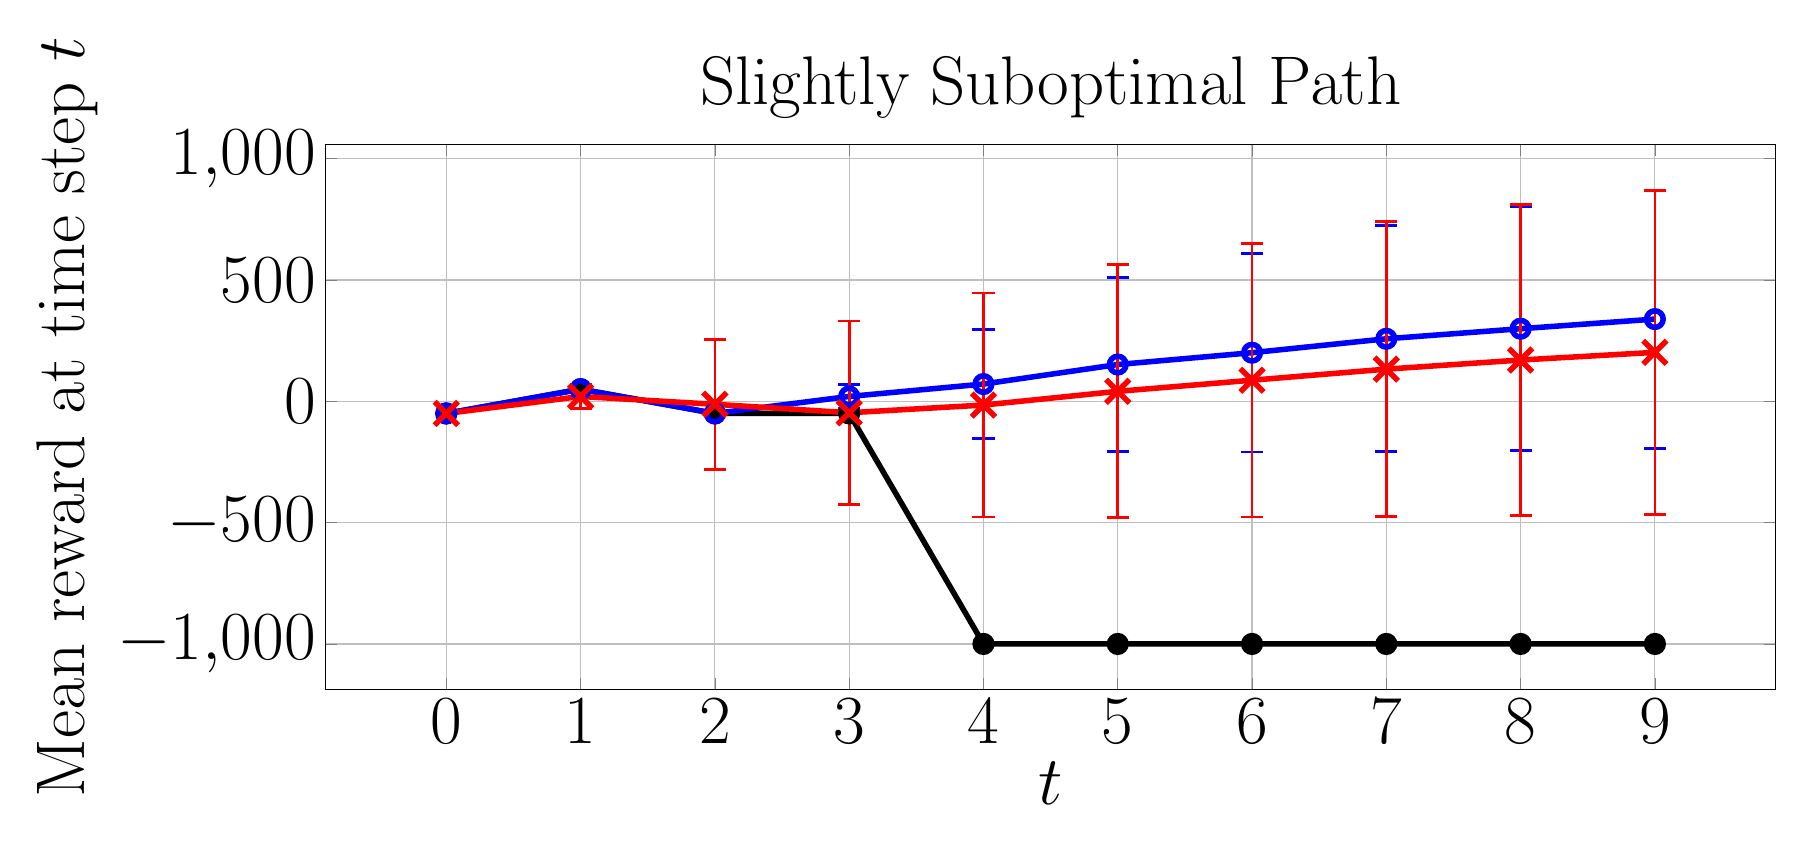
\begin{tikzpicture}
                \begin{axis}[
                    xlabel={$t$},
                    ylabel={Mean reward at time step $t$},
                    title={Slightly Suboptimal Path},
                    grid=both,
                    width=20cm, height=8.5cm,
                    every axis/.style={font=\Huge},
                    %
                ]
               \addplot[
                    color=black, %
                    mark=*, %
                    line width=2pt,
                    mark size=3pt,
                ]
                coordinates {
                    (0, -50.0)
                    (1, 50.0)
                    (2, -50.0)
                    (3, -50.0)
                    (4, -1000.0)
                    (5, -1000.0)
                    (6, -1000.0)
                    (7, -1000.0)
                    (8, -1000.0)
                    (9, -1000.0)
                };
                %
                \addplot[
                    color=blue, %
                    mark=o, %
                    line width=2pt,
                    mark size=3pt,
                    error bars/.cd,
                    y dir=both, %
                    y explicit, %
                    error bar style={line width=1pt,solid},
                    error mark options={line width=1pt,mark size=4pt,rotate=90}
                ]
                coordinates {
                    (0, -50.0)  +- (0, 0.0)
                    (1, 50.0)  +- (0, 0.0) 
                    (2, -50.0)  +- (0, 0.0) 
                    (3, 20.0631)  +- (0, 49.97539413)
                    (4, 71.206585)  +- (0, 226.02033693)
                    (5, 151.60797) +- (0, 359.23292559)
                    (6, 200.40593) +- (0, 408.86185176)
                    (7, 257.77948) +- (0, 466.10372804)
                    (8, 299.237465) +- (0, 501.82579506)
                    (9, 338.9129) +- (0, 532.06124996)
                };
                %
                \addplot[
                    color=red, %
                    mark=x, %
                    line width=2pt,
                    mark size=6pt,
                    error bars/.cd,
                    y dir=both, %
                    y explicit, %
                    error bar style={line width=1pt,solid},
                    error mark options={line width=1pt,mark size=4pt,rotate=90}
                ]
                coordinates {
                    (0, -50.0)  +- (0, 0.0)
                    (1, 20.00736)  +- (0, 49.99786741) 
                    (2, -12.282865)  +- (0, 267.598755) 
                    (3, -47.125995)  +- (0, 378.41755832)
                    (4, -15.381965)  +- (0, 461.77616558)
                    (5, 41.15459) +- (0, 521.53189262)
                    (6, 87.01595) +- (0, 564.22243126 )
                    (7, 132.62376) +- (0, 607.31338037)
                    (8, 170.168145) +- (0, 641.48013693)
                    (9, 201.813135) +- (0, 667.29441777)
                };
                %
                %
                %
                %
                %
                %
                %
                %
                %
                %
                %
                %
                %
                %
                %
                %
                %
                %
                %
                \end{axis}
            \end{tikzpicture}
         }
    }\\[-1.5pt]
    \subfigure[\footnotesize Lowest cumulative reward: Interval CFMDP ($100$), Gumbel-max SCM ($100$)]{%
         \resizebox{0.76\columnwidth}{!}{
             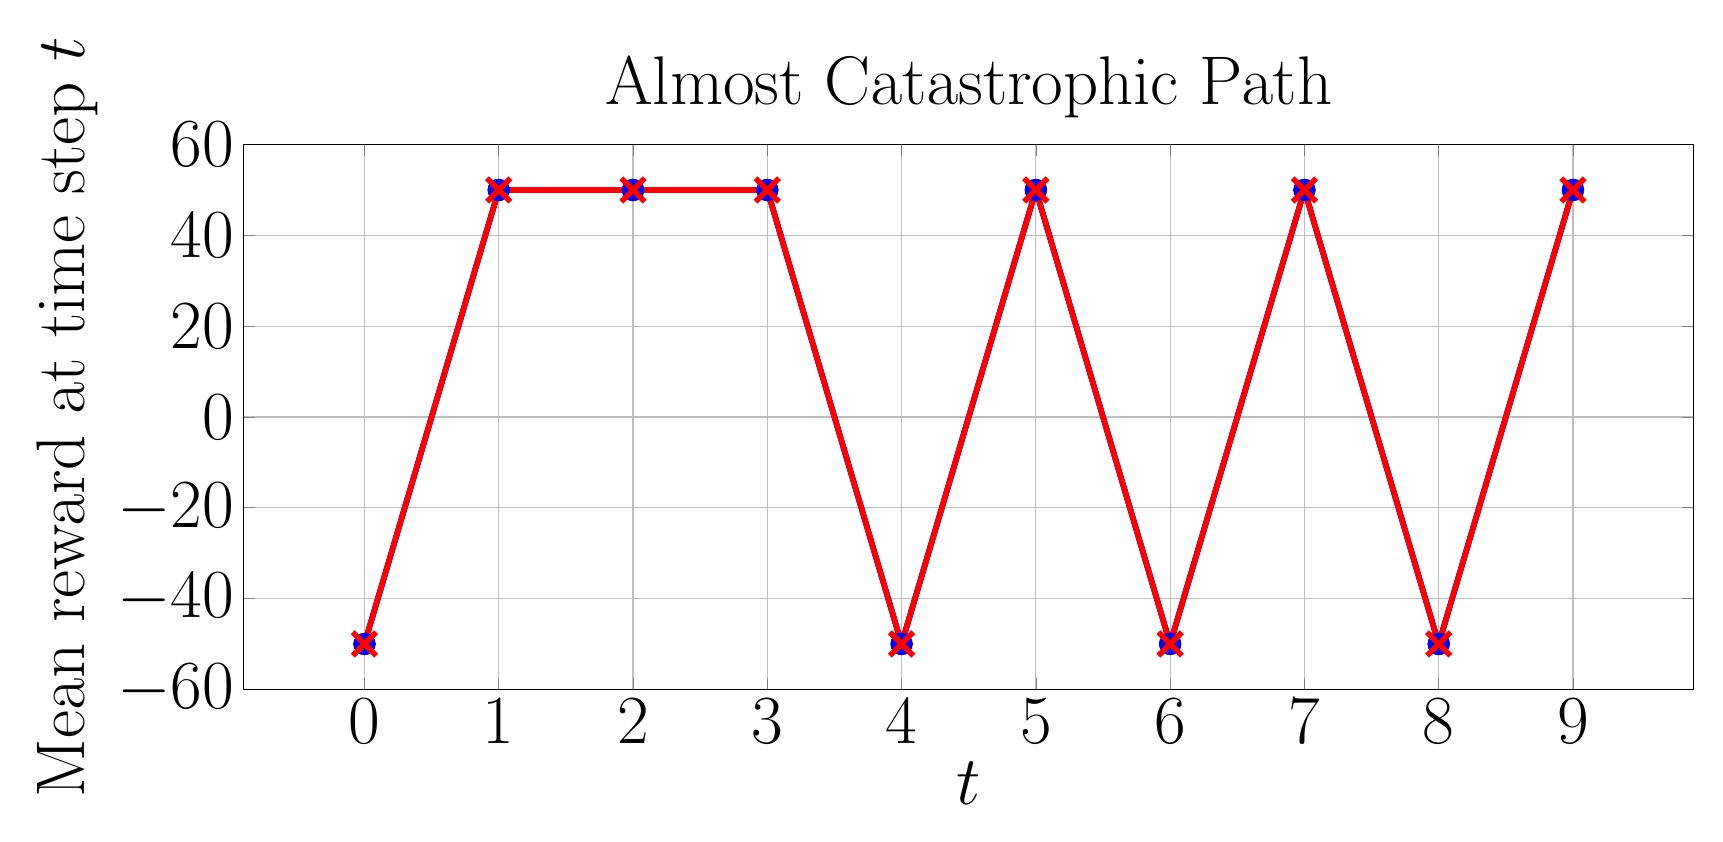
\begin{tikzpicture}
                \begin{axis}[
                    xlabel={$t$},
                    ylabel={Mean reward at time step $t$},
                    title={Almost Catastrophic Path},
                    grid=both,
                    every axis/.style={font=\Huge},
                    width=20cm, height=8.5cm,
                    %
                ]
               \addplot[
                    color=black, %
                    mark=*, %
                    line width=2pt,
                    mark size=3pt,
                ]
                coordinates {
                    (0, -50.0)
                    (1, 50.0)
                    (2, 50.0)
                    (3, 50.0)
                    (4, -50.0)
                    (5, 50.0)
                    (6, -50.0)
                    (7, 50.0)
                    (8, -50.0)
                    (9, 50.0)
                };
                %
                %
                \addplot[
                    color=blue, %
                    mark=o, %
                    line width=2pt,
                    mark size=3pt,
                    error bars/.cd,
                    y dir=both, %
                    y explicit, %
                    error bar style={line width=1pt,solid},
                    error mark options={line width=1pt,mark size=4pt,rotate=90}
                ]
                coordinates {
                    (0, -50.0)  +- (0, 0.0)
                    (1, 50.0)  +- (0, 0.0) 
                    (2, 50.0)  +- (0, 0.0) 
                    (3, 50.0)  +- (0, 0.0)
                    (4, -50.0)  +- (0, 0.0)
                    (5, 50.0) +- (0, 0.0)
                    (6, -50.0) +- (0, 0.0)
                    (7, 50.0) +- (0, 0.0)
                    (8, -50.0) +- (0, 0.0)
                    (9, 50.0) +- (0, 0.0)
                };
                %
                \addplot[
                    color=red, %
                    mark=x, %
                    line width=2pt,
                    mark size=6pt,
                    error bars/.cd,
                    y dir=both, %
                    y explicit, %
                    error bar style={line width=1pt,solid},
                    error mark options={line width=1pt,mark size=4pt,rotate=90}
                ]
                coordinates {
                    (0, -50.0)  +- (0, 0.0)
                    (1, 50.0)  +- (0, 0.0) 
                    (2, 50.0)  +- (0, 0.0) 
                    (3, 50.0)  +- (0, 0.0)
                    (4, -50.0)  +- (0, 0.0)
                    (5, 50.0) +- (0, 0.0)
                    (6, -50.0) +- (0, 0.0)
                    (7, 50.0) +- (0, 0.0)
                    (8, -50.0) +- (0, 0.0)
                    (9, 50.0) +- (0, 0.0)
                };
                %
                %
                %
                %
                %
                %
                %
                %
                %
                %
                %
                %
                %
                %
                %
                %
                %
                %
                %
                \end{axis}
            \end{tikzpicture}
         }
    }
    \hspace{1cm}
    \subfigure[\footnotesize Lowest cumulative reward: Interval CFMDP ($-7150$), Gumbel-max SCM ($-9050$)]{%
         \resizebox{0.76\columnwidth}{!}{
            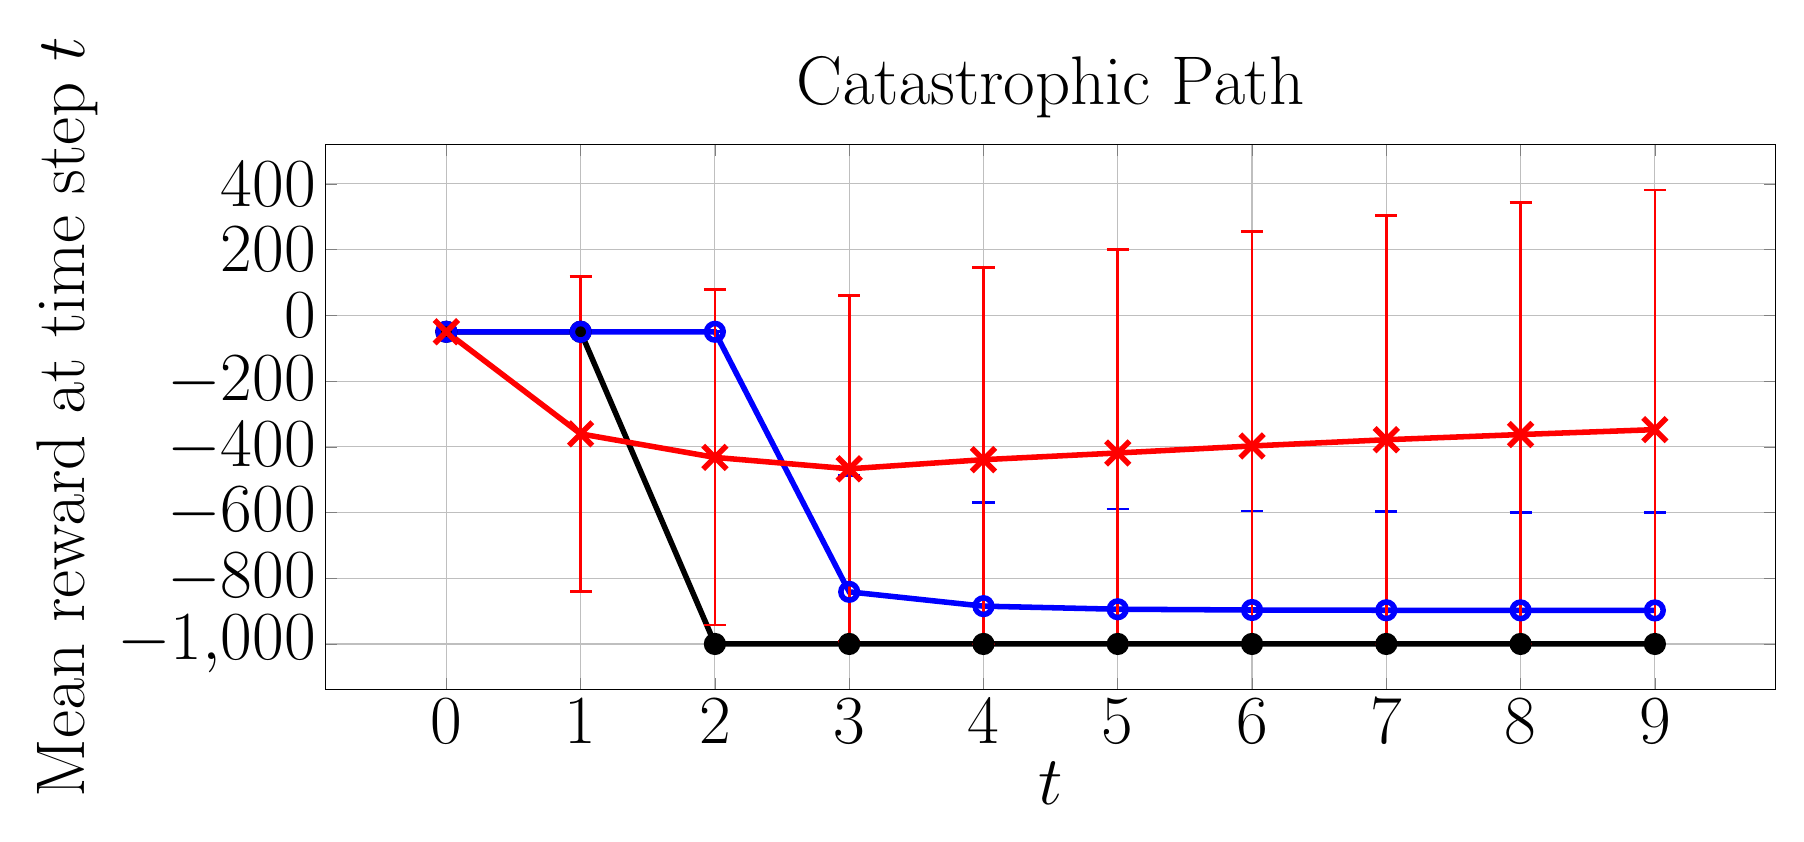
\begin{tikzpicture}
                \begin{axis}[
                    xlabel={$t$},
                    ylabel={Mean reward at time step $t$},
                    title={Catastrophic Path},
                    grid=both,
                    width=20cm, height=8.5cm,
                    every axis/.style={font=\Huge},
                    %
                ]
               \addplot[
                    color=black, %
                    mark=*, %
                    line width=2pt,
                    mark size=3pt,
                ]
                coordinates {
                    (0, -50.0)
                    (1, -50.0)
                    (2, -1000.0)
                    (3, -1000.0)
                    (4, -1000.0)
                    (5, -1000.0)
                    (6, -1000.0)
                    (7, -1000.0)
                    (8, -1000.0)
                    (9, -1000.0)
                };
                %
                %
                \addplot[
                    color=blue, %
                    mark=o, %
                    line width=2pt,
                    mark size=3pt,
                    error bars/.cd,
                    y dir=both, %
                    y explicit, %
                    error bar style={line width=1pt,solid},
                    error mark options={line width=1pt,mark size=4pt,rotate=90}
                ]
                coordinates {
                    (0, -50.0)  +- (0, 0.0)
                    (1, -50.0)  +- (0, 0.0) 
                    (2, -50.0)  +- (0, 0.0) 
                    (3, -841.440725)  += (0, 354.24605512) -= (0, 158.559275)
                    (4, -884.98225)  += (0, 315.37519669) -= (0, 115.01775)
                    (5, -894.330425) += (0, 304.88572805) -= (0, 105.669575)
                    (6, -896.696175) += (0, 301.19954514) -= (0, 103.303825)
                    (7, -897.4635) += (0, 299.61791279) -= (0, 102.5365)
                    (8, -897.77595) += (0, 298.80392585) -= (0, 102.22405)
                    (9, -897.942975) += (0, 298.32920557) -= (0, 102.057025)
                };
                %
                \addplot[
                    color=red, %
                    mark=x, %
                    line width=2pt,
                    mark size=6pt,
                    error bars/.cd,
                    y dir=both, %
                    y explicit, %
                    error bar style={line width=1pt,solid},
                    error mark options={line width=1pt,mark size=4pt,rotate=90}
                ]
            coordinates {
                    (0, -50.0)  +- (0, 0.0)
                    (1, -360.675265)  +- (0, 479.39812699) 
                    (2, -432.27629)  +- (0, 510.38620897) 
                    (3, -467.029545)  += (0, 526.36009628) -= (0, 526.36009628)
                    (4, -439.17429)  += (0, 583.96638919) -= (0, 560.82571)
                    (5, -418.82704) += (0, 618.43027478) -= (0, 581.17296)
                    (6, -397.464895) += (0, 652.67322574) -= (0, 602.535105)
                    (7, -378.49052) += (0, 682.85407033) -= (0, 621.50948)
                    (8, -362.654195) += (0, 707.01412023) -= (0, 637.345805)
                    (9, -347.737935) += (0, 729.29076479) -= (0, 652.262065)
                };
                %
                %
                %
                %
                %
                %
                %
                %
                %
                %
                %
                %
                %
                %
                %
                %
                %
                %
                %
                \end{axis}
            \end{tikzpicture}
         }
    }
    \caption{Average instant reward of CF paths induced by policies on Sepsis.}
    \label{fig: reward sepsis}
\end{figure*}

%
%
%
\subsection{Interval CFMDP Bounds}
%
%
Table \ref{tab:nonzero_probs} presents the mean counterfactual probability bound widths (excluding transitions where the upper bound is $0$) for each MDP, averaged over 20 observed paths. We compare the bounds under counterfactual stability (CS) and monotonicity (M) assumptions, CS alone, and no assumptions. This shows that the assumptions marginally reduce the bound widths, indicating the assumptions tighten the bounds without excluding too many causal models, as intended.
\renewcommand{\arraystretch}{1}

\begin{table}
\centering
\caption{Mean width of counterfactual probability bounds}
\resizebox{0.8\columnwidth}{!}{%
\begin{tabular}{|c|c|c|c|}
\hline
\multirow{2}{*}{\textbf{Environment}} & \multicolumn{3}{c|}{\textbf{Assumptions}} \\ \cline{2-4}
 & \textbf{CS + M} & \textbf{CS} & \textbf{None\tablefootnote{\jl{Equivalent to \citet{li2024probabilities}'s bounds (see Section \ref{sec: equivalence with Li}).}}} \\ \hline
\textbf{GridWorld} ($p=0.9$) & 0.0817 & 0.0977 & 0.100 \\ \hline
\textbf{GridWorld} ($p=0.4$) & 0.552  & 0.638  & 0.646 \\ \hline
\textbf{Sepsis} & 0.138 & 0.140 & 0.140 \\ \hline
\end{tabular}
}
\label{tab:nonzero_probs}
\end{table}


\subsection{Execution Times}
Table \ref{tab: times} compares the average time needed to generate the interval CFMDP vs.\ the Gumbel-max SCM CFMDP for 20 observations.
The GridWorld algorithms were run single-threaded, while the Sepsis experiments were run in parallel.
Generating the interval CFMDP is significantly faster as it uses exact analytical bounds, whereas the Gumbel-max CFMDP requires sampling from the Gumbel distribution to estimate counterfactual transition probabilities. \jl{Since constructing the counterfactual MDP models is the main bottleneck in both approaches, ours is more efficient overall and suitable for larger MDPs.}
\begin{table}
\centering
\caption{Mean execution time to generate CFMDPs}
\resizebox{0.99\columnwidth}{!}{%
\begin{tabular}{|c|c|c|}
\hline
\multirow{2}{*}{\textbf{Environment}} & \multicolumn{2}{c|}{\textbf{Mean Execution Time (s)}} \\ \cline{2-3} 
                                      & \textbf{Interval CFMDP} & \textbf{Gumbel-max CFMDP} \\ \hline
\textbf{GridWorld ($p=0.9$) }                  & 0.261                   & 56.1                      \\ \hline
\textbf{GridWorld ($p=0.4$)  }                 & 0.336                   & 54.5                      \\ \hline
\textbf{Sepsis}                                 & 688                     & 2940                      \\ \hline
\end{tabular}%
}
\label{tab: times}
\end{table}

\section{Discussion of Assumptions}\label{sec:discussion}
In this paper, we have made several assumptions for the sake of clarity and simplicity. In this section, we discuss the rationale behind these assumptions, the extent to which these assumptions hold in practice, and the consequences for our protocol when these assumptions hold.

\subsection{Assumptions on the Demand}

There are two simplifying assumptions we make about the demand. First, we assume the demand at any time is relatively small compared to the channel capacities. Second, we take the demand to be constant over time. We elaborate upon both these points below.

\paragraph{Small demands} The assumption that demands are small relative to channel capacities is made precise in \eqref{eq:large_capacity_assumption}. This assumption simplifies two major aspects of our protocol. First, it largely removes congestion from consideration. In \eqref{eq:primal_problem}, there is no constraint ensuring that total flow in both directions stays below capacity--this is always met. Consequently, there is no Lagrange multiplier for congestion and no congestion pricing; only imbalance penalties apply. In contrast, protocols in \cite{sivaraman2020high, varma2021throughput, wang2024fence} include congestion fees due to explicit congestion constraints. Second, the bound \eqref{eq:large_capacity_assumption} ensures that as long as channels remain balanced, the network can always meet demand, no matter how the demand is routed. Since channels can rebalance when necessary, they never drop transactions. This allows prices and flows to adjust as per the equations in \eqref{eq:algorithm}, which makes it easier to prove the protocol's convergence guarantees. This also preserves the key property that a channel's price remains proportional to net money flow through it.

In practice, payment channel networks are used most often for micro-payments, for which on-chain transactions are prohibitively expensive; large transactions typically take place directly on the blockchain. For example, according to \cite{river2023lightning}, the average channel capacity is roughly $0.1$ BTC ($5,000$ BTC distributed over $50,000$ channels), while the average transaction amount is less than $0.0004$ BTC ($44.7k$ satoshis). Thus, the small demand assumption is not too unrealistic. Additionally, the occasional large transaction can be treated as a sequence of smaller transactions by breaking it into packets and executing each packet serially (as done by \cite{sivaraman2020high}).
Lastly, a good path discovery process that favors large capacity channels over small capacity ones can help ensure that the bound in \eqref{eq:large_capacity_assumption} holds.

\paragraph{Constant demands} 
In this work, we assume that any transacting pair of nodes have a steady transaction demand between them (see Section \ref{sec:transaction_requests}). Making this assumption is necessary to obtain the kind of guarantees that we have presented in this paper. Unless the demand is steady, it is unreasonable to expect that the flows converge to a steady value. Weaker assumptions on the demand lead to weaker guarantees. For example, with the more general setting of stochastic, but i.i.d. demand between any two nodes, \cite{varma2021throughput} shows that the channel queue lengths are bounded in expectation. If the demand can be arbitrary, then it is very hard to get any meaningful performance guarantees; \cite{wang2024fence} shows that even for a single bidirectional channel, the competitive ratio is infinite. Indeed, because a PCN is a decentralized system and decisions must be made based on local information alone, it is difficult for the network to find the optimal detailed balance flow at every time step with a time-varying demand.  With a steady demand, the network can discover the optimal flows in a reasonably short time, as our work shows.

We view the constant demand assumption as an approximation for a more general demand process that could be piece-wise constant, stochastic, or both (see simulations in Figure \ref{fig:five_nodes_variable_demand}).
We believe it should be possible to merge ideas from our work and \cite{varma2021throughput} to provide guarantees in a setting with random demands with arbitrary means. We leave this for future work. In addition, our work suggests that a reasonable method of handling stochastic demands is to queue the transaction requests \textit{at the source node} itself. This queuing action should be viewed in conjunction with flow-control. Indeed, a temporarily high unidirectional demand would raise prices for the sender, incentivizing the sender to stop sending the transactions. If the sender queues the transactions, they can send them later when prices drop. This form of queuing does not require any overhaul of the basic PCN infrastructure and is therefore simpler to implement than per-channel queues as suggested by \cite{sivaraman2020high} and \cite{varma2021throughput}.

\subsection{The Incentive of Channels}
The actions of the channels as prescribed by the DEBT control protocol can be summarized as follows. Channels adjust their prices in proportion to the net flow through them. They rebalance themselves whenever necessary and execute any transaction request that has been made of them. We discuss both these aspects below.

\paragraph{On Prices}
In this work, the exclusive role of channel prices is to ensure that the flows through each channel remains balanced. In practice, it would be important to include other components in a channel's price/fee as well: a congestion price  and an incentive price. The congestion price, as suggested by \cite{varma2021throughput}, would depend on the total flow of transactions through the channel, and would incentivize nodes to balance the load over different paths. The incentive price, which is commonly used in practice \cite{river2023lightning}, is necessary to provide channels with an incentive to serve as an intermediary for different channels. In practice, we expect both these components to be smaller than the imbalance price. Consequently, we expect the behavior of our protocol to be similar to our theoretical results even with these additional prices.

A key aspect of our protocol is that channel fees are allowed to be negative. Although the original Lightning network whitepaper \cite{poon2016bitcoin} suggests that negative channel prices may be a good solution to promote rebalancing, the idea of negative prices in not very popular in the literature. To our knowledge, the only prior work with this feature is \cite{varma2021throughput}. Indeed, in papers such as \cite{van2021merchant} and \cite{wang2024fence}, the price function is explicitly modified such that the channel price is never negative. The results of our paper show the benefits of negative prices. For one, in steady state, equal flows in both directions ensure that a channel doesn't loose any money (the other price components mentioned above ensure that the channel will only gain money). More importantly, negative prices are important to ensure that the protocol selectively stifles acyclic flows while allowing circulations to flow. Indeed, in the example of Section \ref{sec:flow_control_example}, the flows between nodes $A$ and $C$ are left on only because the large positive price over one channel is canceled by the corresponding negative price over the other channel, leading to a net zero price.

Lastly, observe that in the DEBT control protocol, the price charged by a channel does not depend on its capacity. This is a natural consequence of the price being the Lagrange multiplier for the net-zero flow constraint, which also does not depend on the channel capacity. In contrast, in many other works, the imbalance price is normalized by the channel capacity \cite{ren2018optimal, lin2020funds, wang2024fence}; this is shown to work well in practice. The rationale for such a price structure is explained well in \cite{wang2024fence}, where this fee is derived with the aim of always maintaining some balance (liquidity) at each end of every channel. This is a reasonable aim if a channel is to never rebalance itself; the experiments of the aforementioned papers are conducted in such a regime. In this work, however, we allow the channels to rebalance themselves a few times in order to settle on a detailed balance flow. This is because our focus is on the long-term steady state performance of the protocol. This difference in perspective also shows up in how the price depends on the channel imbalance. \cite{lin2020funds} and \cite{wang2024fence} advocate for strictly convex prices whereas this work and \cite{varma2021throughput} propose linear prices.

\paragraph{On Rebalancing} 
Recall that the DEBT control protocol ensures that the flows in the network converge to a detailed balance flow, which can be sustained perpetually without any rebalancing. However, during the transient phase (before convergence), channels may have to perform on-chain rebalancing a few times. Since rebalancing is an expensive operation, it is worthwhile discussing methods by which channels can reduce the extent of rebalancing. One option for the channels to reduce the extent of rebalancing is to increase their capacity; however, this comes at the cost of locking in more capital. Each channel can decide for itself the optimum amount of capital to lock in. Another option, which we discuss in Section \ref{sec:five_node}, is for channels to increase the rate $\gamma$ at which they adjust prices. 

Ultimately, whether or not it is beneficial for a channel to rebalance depends on the time-horizon under consideration. Our protocol is based on the assumption that the demand remains steady for a long period of time. If this is indeed the case, it would be worthwhile for a channel to rebalance itself as it can make up this cost through the incentive fees gained from the flow of transactions through it in steady state. If a channel chooses not to rebalance itself, however, there is a risk of being trapped in a deadlock, which is suboptimal for not only the nodes but also the channel.

\section{Conclusion}
This work presents DEBT control: a protocol for payment channel networks that uses source routing and flow control based on channel prices. The protocol is derived by posing a network utility maximization problem and analyzing its dual minimization. It is shown that under steady demands, the protocol guides the network to an optimal, sustainable point. Simulations show its robustness to demand variations. The work demonstrates that simple protocols with strong theoretical guarantees are possible for PCNs and we hope it inspires further theoretical research in this direction.
\section{Conclusion}
In this work, we propose a simple yet effective approach, called SMILE, for graph few-shot learning with fewer tasks. Specifically, we introduce a novel dual-level mixup strategy, including within-task and across-task mixup, for enriching the diversity of nodes within each task and the diversity of tasks. Also, we incorporate the degree-based prior information to learn expressive node embeddings. Theoretically, we prove that SMILE effectively enhances the model's generalization performance. Empirically, we conduct extensive experiments on multiple benchmarks and the results suggest that SMILE significantly outperforms other baselines, including both in-domain and cross-domain few-shot settings.
% \smallskip
% \myparagraph{Acknowledgments} We thank the reviewers for their comments.
% The work by Moshe Tennenholtz was supported by funding from the
% European Research Council (ERC) under the European Union's Horizon
% 2020 research and innovation programme (grant agreement 740435).


\bibliographystyle{plain}  % 根据需要选择合适的参考文献样式
\bibliography{references}

\end{document}
